%%%%%%%%%%%%%%%%%%%%%%%%%%%%%%%%%%%%%%%%%%%%%%%%%%%%%%%%%%%%%%%%%%%%%%
%%  disstemplate.tex, to be compiled with latex.		     %
%%  08 April 2002	Version 4				     %
%%%%%%%%%%%%%%%%%%%%%%%%%%%%%%%%%%%%%%%%%%%%%%%%%%%%%%%%%%%%%%%%%%%%%%
%%								     %
%%  Writing a Doctoral Dissertation with LaTeX at		     %
%%	the University of Texas at Austin			     %
%%								     %
%%  (Modify this ``template'' for your own dissertation.)	     %
%%								     %
%%%%%%%%%%%%%%%%%%%%%%%%%%%%%%%%%%%%%%%%%%%%%%%%%%%%%%%%%%%%%%%%%%%%%%


\documentclass[12pt]{report}	% The documentclass must be ``report''.

\usepackage{utdiss2}  		% Dissertation package style file.


%%%%%%%%%%%%%%%%%%%%%%%%%%%%%%%%%%%%%%%%%%%%%%%%%%%%%%%%%%%%%%%%%%%%%%
% Optional packages used for this sample dissertation. If you don't  %
% need a capability in your dissertation, feel free to comment out   %
% the package usage command.					     %
%%%%%%%%%%%%%%%%%%%%%%%%%%%%%%%%%%%%%%%%%%%%%%%%%%%%%%%%%%%%%%%%%%%%%%

\usepackage{amsmath,amsthm,amsfonts,amscd} 
% Some packages to write mathematics.
\usepackage{eucal} 	 	% Euler fonts
\usepackage{verbatim}      	% Allows quoting source with commands.
\usepackage{makeidx}       	% Package to make an index.
\usepackage{epsfig}         	% Allows inclusion of eps files.
\usepackage{url}		% Allows good typesetting of web URLs.
\usepackage{amsmath}
\usepackage[fleqn]{mathtools}
\usepackage{amssymb}
\usepackage{amsthm}
\usepackage{enumitem}
\usepackage{float}
\usepackage{subcaption}
\usepackage[linesnumbered,ruled]{algorithm2e}
\usepackage{xcolor}
\usepackage{adjustbox}
\usepackage{tabularx}
\newcolumntype{L}{>{\raggedright\arraybackslash}X}
%\usepackage{draftcopy}		% Uncomment this line to have the
% word, "DRAFT," as a background
% "watermark" on all of the pages of
% of your draft versions. When ready
% to generate your final copy, re-comment
% it out with a percent sign to remove
% the word draft before you re-run
% Makediss for the last time.

\author{Brian French}  	% Required

\address{2900 Swisher St, Austin TX}  % Required

\title{Post-Disaster Repair and Resilient Modeling for Power Grids with Road Network Considerations}
% Required

%%%%%%%%%%%%%%%%%%%%%%%%%%%%%%%%%%%%%%%%%%%%%%%%%%%%%%%%%%%%%%%%%%%%%%
% NOTICE: The total number of supervisors and other members %%%%%%%%%%
%%%%%%%%%%%%%%% MUST be seven (7) or less! If you put in more, %%%%%%%
%%%%%%%%%%%%%%% they are put on the page after the Committee %%%%%%%%%
%%%%%%%%%%%%%%% Certification of Approved Version page. %%%%%%%%%%%%%%
%%%%%%%%%%%%%%%%%%%%%%%%%%%%%%%%%%%%%%%%%%%%%%%%%%%%%%%%%%%%%%%%%%%%%%

%%%%%%%%%%%%%%%%%%%%%%%%%%%%%%%%%%%%%%%%%%%%%%%%%%%%%%%%%%%%%%%%%%%%%%
%
% Enter names of the supervisor and co-supervisor(s), if any,
% of your dissertation committee. Put one name per line with
% the name in square brackets. The name on the last line, however,
% must be in curly braces.
%
% If you have only one supervisor, the entry below will read:
%
%	\supervisor
%		{Supervisor's Name}
%
% NOTE: Maximum three supervisors. Minimum one supervisor.
% NOTE: The Office of Graduate Studies will accept only two supervisors!
% 
%
\supervisor
{Erhan Kutanoglu}
%%%%%%%%%%%%%%%%%%%%%%%%%%%%%%%%%%%%%%%%%%%%%%%%%%%%%%%%%%%%%%%%%%%%%%
%
% Enter names of the other (non-supervisor) members(s) of your
% dissertation committee. Put one name per line with the name
% in square brackets. The name on the last line, however, must
% be in curly braces.
%
% NOTE: Maximum six other members. Minimum zero other members.
% NOTE: The Office of Graduate Studies may restrict you to a total
%	of six committee members.
%
%
\committeemembers
{Surya Santoso}


%%%%%%%%%%%%%%%%%%%%%%%%%%%%%%%%%%%%%%%%%%%%%%%%%%%%%%%%%%%%%%%%%%%%%%

\previousdegrees{B.S.}
% The abbreviated form of your previous degree(s).
% E.g., \previousdegrees{B.S., MBA}.
%
% The default value is `B.S., M.S.'

%\graduationmonth{...}      
% Graduation month, either May, August, or December, in the form
% as `\graduationmonth{May}'. Do not abbreviate.
%
% The default value (either May, August, or December) is guessed
% according to the time of running LaTeX.

%\graduationyear{...}   
% Graduation year, in the form as `\graduationyear{2001}'.
% Use a 4 digit (not a 2 digit) number.
%
% The default value is guessed according to the time of 
% running LaTeX.

%\typist{...}       
% The name(s) of typist(s), put `the author' if you do it yourself.
% E.g., `\typist{Maryann Hersey and the author}'.
%
% The default value is `the author'.


%%%%%%%%%%%%%%%%%%%%%%%%%%%%%%%%%%%%%%%%%%%%%%%%%%%%%%%%%%%%%%%%%%%%%%
% Commands for master's theses and reports.			     %
%%%%%%%%%%%%%%%%%%%%%%%%%%%%%%%%%%%%%%%%%%%%%%%%%%%%%%%%%%%%%%%%%%%%%%
%
% If the degree you're seeking is NOT Doctor of Philosophy, uncomment
% (remove the % in front of) the following two command lines (the ones
% that have the \ as their second character).
%
\degree{MASTER OF Science}
\degreeabbr{M.S.}

% Uncomment the line below that corresponds to the type of master's
% document you are writing.
%
%\masterreport
\masterthesis


%%%%%%%%%%%%%%%%%%%%%%%%%%%%%%%%%%%%%%%%%%%%%%%%%%%%%%%%%%%%%%%%%%%%%%
% Some optional commands to change the document's defaults.	     %
%%%%%%%%%%%%%%%%%%%%%%%%%%%%%%%%%%%%%%%%%%%%%%%%%%%%%%%%%%%%%%%%%%%%%%
%
%\singlespacing
%\oneandonehalfspacing

%\singlespacequote
\oneandonehalfspacequote

\topmargin 0.125in	% Adjust this value if the PostScript file output
% of your dissertation has incorrect top and 
% bottom margins. Print a copy of at least one
% full page of your dissertation (not the first
% page of a chapter) and measure the top and
% bottom margins with a ruler. You must have
% a top margin of 1.5" and a bottom margin of
% at least 1.25". The page numbers must be at
% least 1.00" from the bottom of the page.
% If the margins are not correct, adjust this
% value accordingly and re-compile and print again.
%
% The default value is 0.125"

% If you want to adjust other margins, they are in the
% utdiss2-nn.sty file near the top. If you are using
% the shell script Makediss on a Unix/Linux system, make
% your changes in the utdiss2-nn.sty file instead of
% utdiss2.sty because Makediss will overwrite any changes
% made to utdiss2.sty.

%%%%%%%%%%%%%%%%%%%%%%%%%%%%%%%%%%%%%%%%%%%%%%%%%%%%%%%%%%%%%%%%%%%%%%
% Some optional commands to be tested.				     %
%%%%%%%%%%%%%%%%%%%%%%%%%%%%%%%%%%%%%%%%%%%%%%%%%%%%%%%%%%%%%%%%%%%%%%

% If there are 10 or more sections, 10 or more subsections for a section,
% etc., you need to make an adjustment to the Table of Contents with the
% command \longtocentry.
%
%\longtocentry 



%%%%%%%%%%%%%%%%%%%%%%%%%%%%%%%%%%%%%%%%%%%%%%%%%%%%%%%%%%%%%%%%%%%%%%
%	Some math support.					     %
%%%%%%%%%%%%%%%%%%%%%%%%%%%%%%%%%%%%%%%%%%%%%%%%%%%%%%%%%%%%%%%%%%%%%%
%
%	Theorem environments (these need the amsthm package)
%
%% \theoremstyle{plain} %% This is the default

\newtheorem{thm}{Theorem}[section]
\newtheorem{cor}[thm]{Corollary}
\newtheorem{lem}[thm]{Lemma}
\newtheorem{prop}[thm]{Proposition}
\newtheorem{ax}{Axiom}

\theoremstyle{definition}
\newtheorem{defn}{Definition}[section]

\theoremstyle{remark}
\newtheorem{rem}{Remark}[section]
\newtheorem*{notation}{Notation}

%\numberwithin{equation}{section}


%%%%%%%%%%%%%%%%%%%%%%%%%%%%%%%%%%%%%%%%%%%%%%%%%%%%%%%%%%%%%%%%%%%%%%
%	Macros.							     %
%%%%%%%%%%%%%%%%%%%%%%%%%%%%%%%%%%%%%%%%%%%%%%%%%%%%%%%%%%%%%%%%%%%%%%
%
%	Here some macros that are needed in this document:


\newcommand{\latexe}{{\LaTeX\kern.125em2%
		\lower.5ex\hbox{$\varepsilon$}}}

\newcommand{\amslatex}{\AmS-\LaTeX{}}

\chardef\bslash=`\\	% \bslash makes a backslash (in tt fonts)
%	p. 424, TeXbook

\newcommand{\cn}[1]{\texttt{\bslash #1}}

\makeatletter		% Starts section where @ is considered a letter
% and thus may be used in commands.
\def\square{\RIfM@\bgroup\else$\bgroup\aftergroup$\fi
	\vcenter{\hrule\hbox{\vrule\@height.6em\kern.6em\vrule}%
		\hrule}\egroup}
\makeatother		% Ends sections where @ is considered a letter.
% Now @ cannot be used in commands.

\makeindex    % Make the index

%%%%%%%%%%%%%%%%%%%%%%%%%%%%%%%%%%%%%%%%%%%%%%%%%%%%%%%%%%%%%%%%%%%%%%
%		The document starts here.			     %
%%%%%%%%%%%%%%%%%%%%%%%%%%%%%%%%%%%%%%%%%%%%%%%%%%%%%%%%%%%%%%%%%%%%%%

\begin{document}
	
	\copyrightpage          % Produces the copyright page.
	
	
	%
	% NOTE: In a doctoral dissertation, the Committee Certification page
	%		(with signatures) is BEFORE the Title page.
	%	In a masters thesis or report, the Signature page
	%		(with signatures) is AFTER the Title page.
	%
	%	If you are writing a masters thesis or report, you MUST REVERSE
	%	the order of the \commcertpage and \titlepage commands below.
	%
	\commcertpage           % Produces the Committee Certification
	%   of Approved Version page (doctoral)
	%   or Signature page (masters).
	%		20 Mar 2002	cwm
	
	\titlepage              % Produces the title page.
	
	
	
	%%%%%%%%%%%%%%%%%%%%%%%%%%%%%%%%%%%%%%%%%%%%%%%%%%%%%%%%%%%%%%%%%%%%%%
	% Dedication and/or epigraph are optional, but must occur here.      %
	%%%%%%%%%%%%%%%%%%%%%%%%%%%%%%%%%%%%%%%%%%%%%%%%%%%%%%%%%%%%%%%%%%%%%%
	%
	\begin{dedication}
		\index{Dedication@\emph{Dedication}}%
		Dedicated to my loving family.
	\end{dedication}
	
	
	\begin{acknowledgments}		% Optional
		\index{Acknowledgments@\emph{Acknowledgments}}%
		I wish to thank the multitudes of people who helped me. This wouldn't have been possible without the support of my advisor Dr. K as well as the dozens of professors and other grad students who helped me see why operations research was an interesting field to study. I also want to thank my friends, both the nerdy online ones scattered across the country and the ones I saw everyday for helping me stay sane during the combination of graduate school, the COVID-19 pandemic, and the process of thesis writing.
	\end{acknowledgments}
	
	
	% The abstract is required. Note the use of ``utabstract'' instead of
	% ``abstract''! This was necessary to fix a page numbering problem.
	% The abstract heading is generated automatically.
	% Do NOT use \begin{abstract} ... \end{abstract}.
	%
	\utabstract
	\index{Abstract}%
	\indent
This thesis fills a gap in modeling literature for considering road networks and power grids jointly. Models are presented for both road network repair as well as power grid repair considering the road network. Multiple frameworks are presented to handle the interactions between the two systems. We also provide lower bound generation and heuristic solution methods. The repair models are then extended to look at resilience and preparation for future disasters.
	
	
	
	\tableofcontents   % Table of Contents will be automatically
	% generated and placed here.
	
	\listoftables      % List of Tables and List of Figures will be placed
	\listoffigures     % here, if applicable.
	
	
	
	%%%%%%%%%%%%%%%%%%%%%%%%%%%%%%%%%%%%%%%%%%%%%%%%%%%%%%%%%%%%%%%%%%%%%%
	% Actual text starts here.					     %
	%%%%%%%%%%%%%%%%%%%%%%%%%%%%%%%%%%%%%%%%%%%%%%%%%%%%%%%%%%%%%%%%%%%%%%
	%
	% Including external files for each chapter makes this document simpler,
	% makes each chapter simpler, and allows for generating test documents
	% with as few as zero chapters (by commenting out the include statements).
	% This allows quicker processing by the Makediss command file in case you
	% are not working on a specific, long and slow to compile chapter. You
	% can even change the chapter order by merely interchanging the order
	% of the include statements (something I found helpful in my own
	% dissertation).
	%
	\chapter{Introduction}
\index{Introduction@\emph{Introduction}}%

\section{Introduction and Motivation}
Hurricanes are a growing concern in the operation of power grids in coastal areas. This is due partly to the increasing density of cities in coastal areas, but also due to climate change causing rising sea levels that may exacerbate impacts of flooding from hurricanes. Combined with the effects of climate change directly, there is also the indirect effect of water warming causing more frequent and more severe hurricanes \cite{MannEA2006}. This phenomenon suggests that careful power grid resilience and planning for hurricanes will be of increased importance in the coming years.

This thesis explores the gap in existing literature where previous efforts have not explicitly considered how multiple networks depended on each other for the logistics of repair, particularly the post-disaster infrastructure recovery interactions between power grid and road networks. For example, to repair a damaged power grid element, the element must be accessible to the crew attempting to repair it. Moreover, the crew will take time to go from one element to the next to repair, affecting the rate of restoration of the power grid's performance during recovery as time is lost in transit. This implies that the road network becomes part of the overall recovery efforts. This includes multiple aspects such as logistics, relief supply delivery, and power grid repair. During a hurricane, the road network will sustain substantial damage from flooding and/or debris on the road surface, which necessitates road grid repairs/clearance as well. To handle the issues of repairing power grids in a way that minimizes the amount of disruption to power service, both types of repairs (road network and power grid) should be considered jointly. To capture the interaction effects of these two networks, we consider the route that repair crews take on the road network as they conduct repairs to either the roads or the power grid. Previous literature does not study this specific interaction as discussed in the section below.

Understanding of repair efforts on power grids begins with understanding the basics of power grid topology. We divide the power grid into transmission and distribution networks. Transmission networks consist of generators, buses/substations, and high voltage connecting lines. Because this side of the grid has multiple sources and sinks, power is not guaranteed to flow in a certain direction. The distribution side of a network begins at the bus/substation level and connects end users of power to the grid as a whole. Because power flows from the substation to the end user in a single source network, these networks are comparatively simpler to model. For the sake of this thesis, we restrict ourselves to the transmission level power grids as distribution grids are simpler at an electrical level as well as being geographically small enough that ignoring the time costs that come from routing the travel of crews leads to a solution that does not stray from optimality very far. In addition, as distribution level damage happens in routine storms, power utilities have a better understanding of how to handle this damage due to experience. The scale of service loss following damage to the power grid is dramatically different in distribution and transmission. Loss of distribution power lines can lead to loss of power service to small segments of a neighborhood while loss of a substation or set of transmission lines can knock out power to several neighborhoods or entire towns depending on the extent of redundancies.


\section{Literature Review}
\subsection{Hurricane Damage Modeling}
When delving into the background literature, no discussion of modeling repair after a hurricane can happen before looking at the literature on damage to power grids from hurricanes. Guikema et al. \cite{GuikemaEA2010} use a model based on negative binomial regression to estimate the number of downed power lines. They combine this with a classification tree that handles flooding and wind speed as a secondary method for estimation of damage severity. Scherb et al. \cite{ScherbEA2015} on the other hand take an approach more rooted in scenario generation and they try to use the peak wind speed and proximity to the eye wall of a hurricane to construct a loss function (a function that maps wind speed onto probability of damage for a given element) for power lines. Figure 1.1  provides an example of the loss function that shows the relationship between probability of varying levels of damage and local peak windspeed during the hurricane. In their figure $\mu$ and $\sigma$ are respectively the mean and standard deviation of number of breakages in a line for each level of damage.

Both of these papers come to the similar conclusion that damage to 40-70\% of the power lines in the network due to wind and thrown debris is common in hurricanes. Damage is geographically distributed based on proximity to the eye-wall of a hurricane, but because hurricanes are frequently hundreds of miles across, damage inside of a single city may appear functionally random due the small geographic area highly similar peak wind speeds. 

\begin{figure}[htbp]
	\centering
	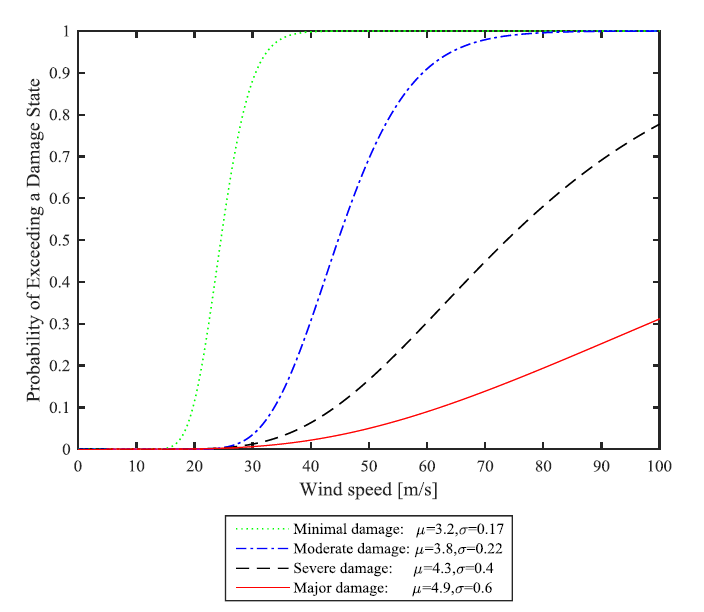
\includegraphics[width=.5\linewidth]{ScherbFigure.PNG}
	\caption{A power line loss function example from \cite{ScherbEA2015}}
\end{figure}

Winkler et al. \cite{WinklerEA2010} provide the most thorough analysis of these 3 papers using real world topographies from various small regions of Texas and generating loss functions for both lines and substations. Worth noting in all three of these examples is that lines and substations sustain the most damage, but generators themselves are robust enough that a hurricane is unlikely to damage them directly, though they may sustain disruption to operations because of disrupted fuel or crew availability. This means they can be treated as undamaged in terms of generation capacity in the modeling in later sections as the generator's functionality depends on its associated substation connecting it to the grid. 
\subsection{Existing Power Grid Repair Modeling}
Repair of power grids in the wake of hurricanes is a reasonably well studied area of research. Ang \cite{NPSMasters} solves a scheduling problem of power grid repair in the wake of both hurricanes and terrorist attacks. The problem is determining in which order should elements be repaired with little consideration of the actual logistics of getting crews to the sites where power grid repair can happen. While they do not consider impacts of roads, they focus on extending repair models to DC power flow based models of the power grid when covering how to model a damaged power grid. Along similar lines, Arab et al. \cite{ArabEA2015} solve a similar problem under uncertainty by treating the state of each power line and generator as a random Bernoulli variable and solving the ensuing stochastic optimization problem. Though it solves the problem as a two stage stochastic program with recourse and treatment of the hurricane damage much closer resembles empirical damage, there is still no consideration of repair logistics, only scheduling and inventory amount. 

Ouyang and Duenas-Osorio \cite{OuyangEA2014} do a statistical analysis of the rate at which damage is recovered in the context of broader power grid resilience. While more descriptive than prescriptive, their analysis concludes that transmission grid repairs take priority alongside ``critical facilities vital to public safety, health, and welfare". Of note in this paper is that their observation that much of the existing literature on repairs to power grid is based on descriptive studies of statistical repair times rather than model-driven optimization models for how to improve that process.

Golari et al. \cite{GolariEA2014} take a different approach to ensuring power demand satisfaction in the context of a damaged power network by approaching the problem in the lens of construction of sub-grids (termed ''islands" in much of the electrical engineering literature) in order to keep demand satisfied. This is done by solving a two stage stochastic program in order to identify the best sub-grids to construct under the uncertainty of a set of contingencies. Islanding is an active field of study in power grid engineering for developing tools to minimize the impact of disaster damage. Panteli et al. \cite{Panteli2016} study disaster damage by constructing islanding plans in a way that would minimize load loss subject to severe weather. Though there is no consideration of repair, their modeling warrants the importance of resilience as an area of study.  A follow on paper to that by Nobels and Panteli \cite{NobelsEA2019} extends the previous work on resilience from islanding  by using IEEE 30 and 57 bus test networks to analysis of cascaded failures caused by disasters. In addition, their modeling differentiates intentional vs unintentional load shedding due to the disaster and corresponding response.
\subsection{Existing Road Grid Repair Modeling}
Pregnolato et al. \cite{PregnolatoEA2017} provide an overview of probability of road damage by location and intensity of damage to the road in terms of flooding and debris. They go on to provide a literature review and meta-analysis of existing papers in this subfield. In addition, the paper summarizes a variety of versions of flooding depth-disruption functions for roads based on local rain intensity. The focus of this paper is not modeling repair efforts as the models provided for road repair are cursory, but the analysis of damage to road networks from debris and flooding in the wake of a disaster is covered in depth.

Looking next at how previous papers have addressed modeling flooding and how to interact with it in a repair context, we start with a paper by Duque et al. \cite{DuqueEA2016}. This paper focuses on distribution of relief supplies, but in the context of the problem of supply distribution the paper considers repair of flooded or damaged roads. Though they solve the problem with dynamic programming rather than the mixed integer programming of similar papers; the idea of repair of roads by traversing them at additional cost is the main contribution of their modeling approach.

Also of note from the perspective of road repair is a paper by Aksu and Ozdamar \cite{AksuEA2014}. Again, it is not a paper focused focused on direct repair of networks, but rather focuses on evacuation and accessibility to areas flooded by the a disaster. This provides additional insight into flooding and relief as well as a different treatment of the problem using mixed integer programming rather than the dynamic programming of Duque et al. Both of these treatments cover short term road clearance in the context of disaster response and relief. 

All three of these papers make similar assumptions in that minor damage to road networks can be repaired in a time horizon relevant to immediate post-disaster response. While more severe damage to roads can require resurfacing or replacement of bridges, debris and flooding clearance is distinct from those repairs.

\subsection{Resilience}
As this thesis deals partly with resilience, we look to the corresponding literature for definitions of resilience in the context of disaster response for power grids. Molyneaux et al. \cite{MolyneauxEA2016} provide a multi-disciplinary literature review of power grid resilience. They broadly define resilience as ``capacity to cope with the unexpected". While they go through multiple measures for resilience they use primarily metrics of price. For example, they reduce power flow to the cost of power and the change in cost from the hurricane damaging the network rather than treating the utility of unsatisfied power demand directly. This approach can be very useful, but it ignores that power is more valuable to some consumers than others in the wake of a hurricane. For example, a hospital restoring power is likely more valuable than a factory restoring power. Panteli and Mancarella \cite{Panteli2017} focus on more specific resilience definitions in the context of disaster response. They focus on both magnitude of drop in service of power demand as well as time dependent total loss of power demand satisfied.

Much of the literature on resilience for power grids comes from study of protecting the power grid from directed attacks. Fortification against a potential terrorist attack is a standard form of study for grid resilience and appears in much of the literature. Relevant among these is a paper by Deka et al. \cite{Deka2018} which provides a study of both initial damage as well as potential damage stemming from cascading failures. In addition, they identify  elements crucial to construction of resilient power networks. More relevant to this thesis is work by Salmeron et al. \cite{Salmeron2004} Their work identifies key elements to make resilient using mixed integer programming based on a DC-powerflow based model of power grids. They solve a bilayer optimization model that involves minimization of the maximum power demand that can be satisfied to determine optimal interdiction. The inner problem how to maximize the amount of power demand that can be serviced given the state of the power grid under damaged operations. The outer problem is therefore how to choose power grid damage in order to make sure that as little demand can be satisfied under ideal operation of the damaged network. This interaction between attacker and defender provides the framework from which they plan resilience.


	
	\chapter{Modeling}
\index{Modeling@\emph{Modeling}}%


\section{Overview}
To motivate the problem, we see both the literature a gap in looking at power grid repairs in a post-disaster context with consideration of the roads as well as specific identification of this problem from government agencies. The Federal Emergency Management Agency's 2017 post season after action report \cite{FEMA2017AAR} and Hurricane Sandy after action report \cite{FEMASandyAAR} identify the lack of coordination between agencies involved in recovery as a major shortcoming and call for increased coordination, particularly for the sake of recovery logistics.

We know from the earlier referenced literature that road repair is a concern in the wake of a hurricane. We assume for the sake of this thesis that all roads can be cleared of flooding and/or debris. Clearing here represents digging out drainage for minor flooding and clearing debris. Severely damaged roads should be treated as completely impassible and dropped from the graph representation of the network to allow this assumption to work in a practical context. While more severely damaged roads are eventually repaired, these repairs frequently represent involved construction efforts spanning weeks or months after a disaster and therefore are beyond the scope of the current modeling efforts.

We model the topology of both power and road networks as a pair of graphs with shared sets of nodes. On the road graph, the nodes are the physical locations of power substations and buses. We abstract away from the roads to a representation of them that captures effects of the road grid existing, but simplifies routing. A more full representation of the road network would include dummy nodes into the road network to represent major intersections, letting the edges/roads represent the shortest paths between those points. This typically comes at the cost of a dramatic increase in runtime as routing-based problems are computationally intense. Therefore we elect to use an abstracted representation based on existing literature on road grid modeling \cite{ChanEA2011} that treats a road network as an abstraction based on frequently traveled paths. 

The nodes representing power substations, generators, and/or buses are mirrored on the power network layer, but the edges at this layer represent the power line connections between substations. This multilayered graph depiction of the two infrastructures allows cleaner mathematical modeling later on. With a given post-disaster damage to both networks (damaged nodes and lines in the power grid and damaged roads in the road network), we analyze of the interactions in the repair efforts needed to get both networks fully operational.

We model time in discrete shifts because it allows for mixed-integer programming to solve both problems in a way where their solutions can be temporally aligned. This temporal alignment allows for interaction frameworks to remain simple.

We assume that direct current (DC) approximations of power flow can accurately approximate the full alternating current (AC) power flow of a real power grid. DC power flow is more accurate than a ``pipe-flow" representation as it captures some of the physics behind electrical flows. This interaction may be important in the consideration of repair and resilience. DC power flow models spread flow out among possible lines whereas pipe-flow style models load all the demand onto single lines due to how they are solved with linear programming since those methods will seek an extreme point solution. DC representation is usually within 5-10\% of the AC power flow solutions \cite{Frank2016} \cite{StottEA2009} making it appropriate for the power repair problem. Since we are considering is one of logistics and not one of power flow management, an approximation of the power flow that relaxes numerical accuracy of power flow but leaves a near optimal repair schedule is justified. We model only the power demand in terms of wattage and not voltage because voltage sag disruptions are a problem primarily at the distribution level \cite{LamoreeEA1994}. Additionally, keeping voltage inside the desired range is a problem of optimal grid control, which is not considered in this thesis \cite{MiretEA2013}.  

With the power grid, we treat distribution below the substation level as a point load associated with a substation. Each substation in real power grid has a distribution level network that services the local area by connecting individual demand such as a house to the power grid as a whole. The wires between substations are considered the transmission level network. The choice to discard the distribution network's topology in the modeling of repair scheduling stems from two factors. First, the distribution network stemming from a substation has geographically co-located damage as distribution areas from a single substation are geographically compact. This implies that including road networks with distribution grid repairs would provide little benefit, as time costs from transiting between one damaged element and another are small. Secondly, flow at the distribution level goes from the substation to the demand sites unlike transmission level networks where flow can go in different directions depending on the state of the grid. This is different from operation of transmission level networks so they can be treated as a point load on the transmission network, avoiding complexity that does not improve insights about the core interaction of concern.

\section{Direct Current Optimal Power Flow (DC-OPF)}
To model repair of damaged power grids, we first must understand the Direct Current-Optimal Power Flow (DC-OPF) model as it forms the basis of all of the more complex power models used in this thesis. The problem can be expressed as satisfying all power demand at minimal generation cost--a problem that shows up frequently in control and analysis of power grids. The power grid can be represented as a graph with edges representing power lines and the nodes of the directed graph corresponding to substations and buses. These substations may service a distribution area with associated unmodeled distribution network. Directionality in the graph is done for bookkeeping as power can flow both directions and by having the graph be directed, we can allow positive flow on edge $(i,j)$ to represent power flow going from $i$ to $j$ and negative flow representing power going from $j$ to $i$. This leads to the nodes representing buses and substations having edges that connect the nodes indexed from lower to higher. For example, edge $(1,2)$ would be included in this modeling, edge $(2,1)$ would not be as it would just be represented as negative flow on edge $(1,2)$.


We use the following notation for clarity in models:
\begin{itemize}
	\item $o(e)$ is the node at the origin of line $e$ 
	\item $d(e)$ is the node at the destination of line $e$
	\item $O(i)$ is the set of lines with origin $i$
	\item $D(i)$ is the set of lines with destination $i$
\end{itemize}
We define the following parameters and sets:
\begin{itemize}
	\item $N$ is the set of nodes indexed by $i$
	\item $E$ is the set of edges indexed by $e$
	\item $C_i$ is the cost of producing one unit (megawatts in this thesis) of power at node $i$
	\item $P_i$ is the maximum power generation in megawatts for node $i$. If there is no generator connected to the substation, maximum production is zero watts.
	\item $D_i$ is the demand for power in megawatts at node $i$
	\item $B_e$ is the line susceptance in per unit siemens for power line $e$ (susceptance is the measure of ease of power flowing along a line)
	\item $\overline{L_e}$ is the maximum amount of flow in megawatts on line $e$
	
\end{itemize}
We also have the following decision variables:
\begin{itemize}
	\item $X_e$ is the power flow on line $e$ 
	\item $Y_i$ is the power generated at node $i$ in megawatts
	\item $\theta_i$ is the phase angle in radians for power flow at node $i$ 
\end{itemize}
The model can then be formulated as follows: 
\begin{equation}
\textnormal{Minimize} \sum_{i\in N} C_i Y_i
\end{equation} 
subject to
\begin{eqnarray}
X_e = B_e (\theta_{o(e)} - \theta_{d(e)}), \hspace{4pt} \forall e \in E\\
Y_i - \sum_{e \in O(i)} X_e + \sum_{e \in D(i)} X_e = D_i, \hspace{4pt} \hspace{4pt} \forall i \in N\\
Y_i \leq P_{i}, \hspace{4pt} \hspace{4pt} \forall i \in N	\\ 
-\overline{L_e} \leq X_e \leq \overline{L_e}, \hspace{4pt} \forall e \in E\\
Y_i \geq 0, \hspace{4pt} \forall i \in N\\
-\pi/2 \leq \theta_i \leq \pi/2, \hspace{4pt} \forall i \in N.
\end{eqnarray}

To explain, the problem is generation power at the minimum cost in a way that satisfies all of the demand subject to the physics of how DC-approximated power grids operate. This problem also solves out line flow amounts and phase angles for each node as expressed in a per unit basis (normalizing everything to the same basis unit such as megawatt). Constraints (2.2) are part of the DC approximation to AC power flow where we assume sin($x$) = $x$ for small values of $x$ and reduce power flow to just its real component (dropping the reactive component of power flow). This representation of power flow tracks only power demand (wattage) and neglects voltage as it is less relevant to this problem, but both versions of DCOPF are a well solved problems in electrical engineering literature \cite{Frank2016} \cite{EldridgeEA2017} \cite{ZhangChow2015}. Constraints (2.3) are a set of standard flow balance constraints that require power going into a node has to be equal to power coming out of node. Constraints (2.4) restrict power generation to the maximum permitted for the generator. Constraints (2.5) model flow capacity for power lines. Constraints (2.6) impose non-negativity limits on generation and constraints (2.7) limit the phase angle to a single period of the sine wave. While overall a simple problem, DCOPF serves as the building block for most of the power grid models used for the rest of this thesis as well as being used in practice for controlling power grid generation and dispatch \cite{LiBo2007}. 
\section{Validating Use of DC Power Flow}

Much of the existing literature in operations research relaxes one step further than DC powerflow all the way to traditional network flow or ``pipe-flow" models that can be used for any abstracted network. For these problems, DC powerflow models are sometimes considered to be unnecessary. This therefore begs the question of why use it over a traditional network flow model. We define traditional network flow to consist of just flow balance and line limits (analogous to relaxation of constraint (2.2) in the DCOPF model below). DC power flow tends to spread power flow out more across lines due to the physics of power flow in a grid while a simpler network flow model tends to seek an extreme point solution, leading to fewer lines under use with heavier loading on those lines as a byproduct of solving it with a linear program. To demonstrate this effect, we solve DCOPF and its corresponding relaxation of constraint (2.2) on IEEE 30 bus and IEEE 57 bus. The results shown in Figure 2.1 show a small but noticeable difference in flow patterns. This may be relevant when modeling system-wide damage in a power grid. Therefore it is worth including in models for repair and resilience. In addition to this, the computational cost of including DC power flow over a pipe-flow model is near zero because extra linear variables have a low impact on runtime of branch-and-bound based solvers. Additionally, this modeling change helps keep math representation of the network closer to the real AC flow, which has the added benefit of making it easier to persuade practitioners in the field that the models presented using DC power flow have relevance to real operations.

\begin{figure}
	\centering
	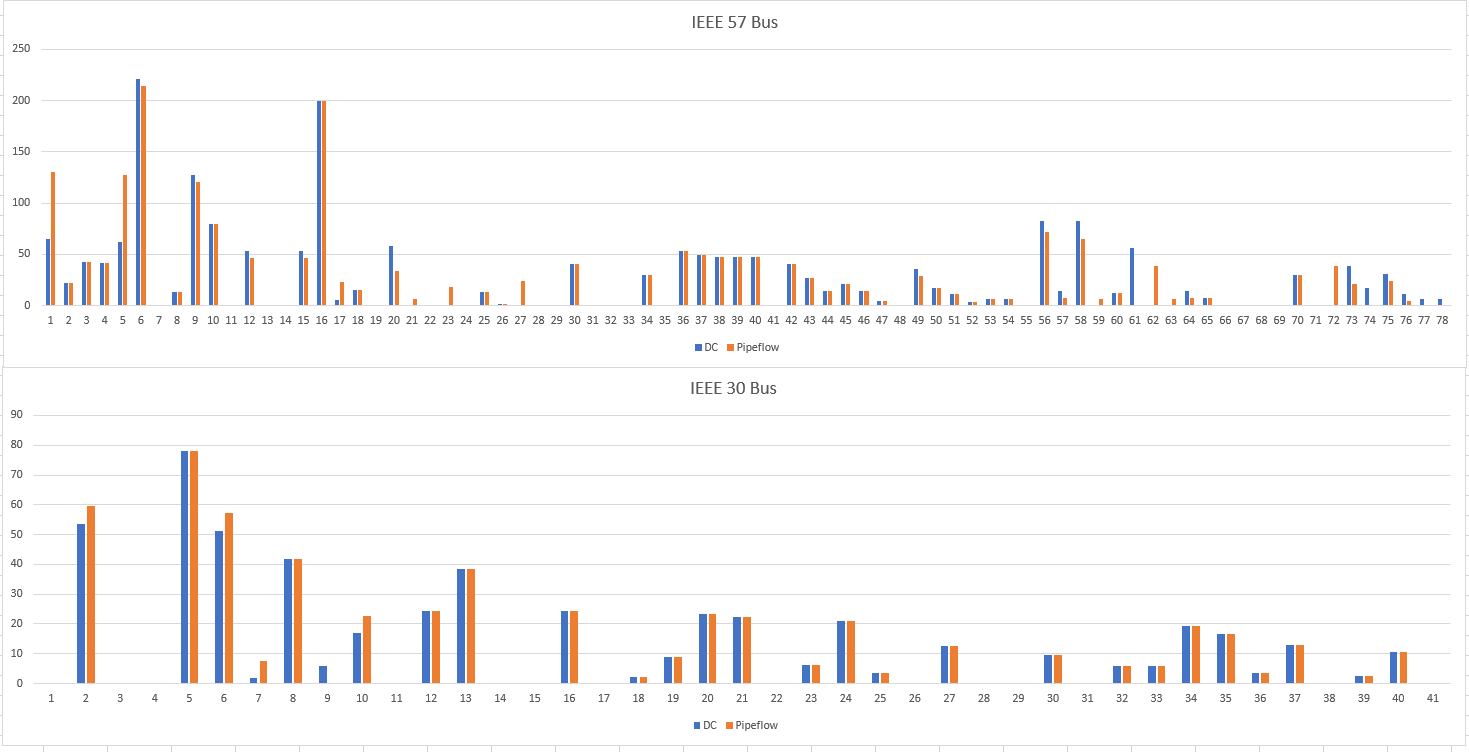
\includegraphics[width=\linewidth]{DCvsPipeflow.PNG}
	\caption{Comparison of DC and traditional (pipeflow) network flow}
\end{figure}

Further, as we extend this model to resilience, use of pipeflow style network models to handle power flow may over-prioritize the resilience of certain lines which strays from optimality on the full AC power grid. Since DC power flow is of low computational cost and low model complexity to add and has upside in some limited cases, we find its inclusion to be warranted.

\section{Road Repair Problem}
When dealing with repairs on the power grid, we need a framework for solving problems based on the damage to the road network. Any framework will rely on a method for modeling repair of the road network. We elect to solve the road repair problem as a scheduling/routing problem for a crew tasked with clearing debris and/or digging out minor flooding, following Duque et al. \cite{DuqueEA2016} and their treatment of how road repairs function. This takes the form of using routing the crew down a damaged road at higher time cost. This is solved by constructing a series of roads to traverse as a tour that begins and ends at a depot in every shift. We model this as follows:

\textbf{Parameters and Sets:}
\begin{itemize}

\item $T$ is the set of time periods (shifts) over the time horizon, indexed by $t$
\item $N$ is the set of nodes in the graph with node 1 being the depot, representing the locations of substations where each substation could have a distribution load, a generator, or both
\item $c_{ij}^t$ is the measure of the value of the road segment from node $i$ to node $j$ during period $t$. $i,j$ pairs that do not have a road between them have value zero.
\item $l_{ij}$ is the transit time in hours of the road segment between nodes $i$ and $j$ under nominal conditions
\item $r_{ij}$ is the time to repair the road segment between nodes $i$ and $j$ (hours), $r_{ij}$>$l_{ij}$ $\forall i,j$ since lines are repaired by transiting them
\item $s^t$ is the length of shift period $t$ in time units (hours)
\item $o_{ij}$ is the initial condition (1 is working, 0 is not) of the road segment between nodes $i$ and $j$
\end{itemize}

\textbf{Decision Variables:}
\begin{itemize}
\item $X_{ij}^t$ is the binary variable for road segment $ij$ being operational in time $t$
\item $Y_{ij}^t$ is the binary variable for travel from $i$ to $j$ being in the tour at time $t$
\item $W_{ij}^t$ is the length of travel time for road segment $ij$ at time $t$
\end{itemize}

Given the parameters and decision variables, we formulate the model as follows:
\begin{equation}
\textnormal{Minimize} \sum_{t \in T}  \sum_{i,j \in N} c_{ij}^t(1-X_{ij}^t) 
\end{equation}
subject to:
\begin{eqnarray}
\sum_{j \in N} Y_{1j}^t = 1,\hspace{6pt} \hspace{6pt} \forall t\in T \\
\sum_{i,j \in N} W_{ij}^t Y_{ij}^t \leq s^t, \hspace{6pt} \forall t\in T \\
W_{ij}^t = \max \{l_{ij}, r_{ij}(1-X_{ij}^t) \}, \hspace{6pt} \forall t\in T, \hspace{5pt} \forall i,j \in N\\
\sum_{j \in N} Y_{ij}^t - \sum_{j \in N} Y_{ji}^t = 0, \hspace{6pt} \forall t\in T, \hspace{5pt} \forall i \in N\\
X_{ij}^t \le \sum_{t'=0}^{t-1} Y_{ij}^{t'} + o_{ij} , \hspace{6pt} \forall t\in \{1,2,....t_{max}\},  \hspace{5pt} \forall i,j \in N\\
\sum_{i,j \in S; i\neq j} Y_{ij}^t \leq |S|-1, \hspace{6pt} \forall S \subset N, \hspace{2pt} S \neq \emptyset, \hspace{5pt} \forall t\in T\\
W_{ij}^t \geq 0, \hspace{5pt} \forall t\in T, \hspace{5pt} \forall i,j \in N \\
X_{ij}^t,Y_{ij}^t, \in \{0,1\}. 
\end{eqnarray}

To explain the modeling, the objective is to minimize the value of out-of-service road. Value here is defined loosely so that without loss of generality, this can be substituted with a set of priority weights from another agency that cares about the road network's operation. For example, the value metric for the road network can be selected based on an agency such as the Red Cross or FEMA that is tasked with bringing relief supplies in to a disaster-stricken area. This modeling is done to capture the issue of both power and road utilities having different priorities when it comes to restoring infrastructure.

Constraints (2.9) force the depot to be in every tour. Constraints (2.10) provide a scheduling constraints that limit the tour's length to the length of the shift. Constraints (2.11) are nonlinear but linearizable constraints that set the length of a road to either its nominal operation time or its repair time depending on whether or not it is marked as working ($X_{ij}^t$ = 1). Constraints (2.12) are standard path connectivity constraints. Constraints (2.13) restrict each road segment to only be working if it started working ($o_{ij}$ = 1) or has been repaired. Constraints (2.14) are a standard set of subtour elimination constraints. Constraints (2.15) and (2.16) exist to restrict decision variables to only valid values.

Of note is that constraints (2.10) and (2.11) are nonlinear as intuitively expressed. We linearize it by rewriting constraints (2.10) and (2.11) as the following:

\begin{eqnarray}
\sum_{i,j \in N} W_{ij}^t \leq s^t, \hspace{6pt} \forall t\in T \\
W_{ij}^t \leq MY_{ij}^t, \hspace{6pt} \forall t\in T, \hspace{5pt} \forall i,j \in N\\
W_{ij}^t \geq l_{ij}Y_{ij}^t, \hspace{6pt} \forall t\in T, \hspace{5pt} \forall i,j \in N\\
W_{ij}^t \geq (1-X_{ij}^t)r_{ij} - (1-Y_{ij}^t)M, \hspace{6pt} \forall t\in T, \hspace{5pt} \forall i,j \in N.
\end{eqnarray}


\section{Power Grid Repair Problem}
When looking at repair of the power grid at the transmission level, we formulate a discrete time mixed integer program that captures both the planning/scheduling/movement of repair crews as well as the DC power flow model. We assume the following:
\begin{itemize}
	\item Repair of a power line can be started from either end of that power line.
	\item Minimum spanning tree's lower bound on the length of a tour/route provides a usable approximation for the sake of keeping model runtime down 
	\item Load shedding can be modeled as a continuous loss even though on real power grids it is a series of discrete decisions to stop power to specific parts of the distribution network that allows for small increments of load to be shed, though not truly continuous power shedding. We make this assumption due the the modeling and computational burden of having many low-impact decisions to make.
	\item Every substation can have an associated demand from an attached distribution network as well as generation capacity from an attached power plant. For substations that do not have these attached, the node demand and/or power generation capacity are set to 0.
\end{itemize}
We pose the model as follows:
\newline
\textbf{Sets and indices:}
\begin{displaymath}
\begin{array}{ll}
N & \mbox{set of nodes, indexed by $i$} \\
E & \mbox{set of power lines, indexed by $e$}\\
R & \mbox{the set of road segments} \\
T & \mbox{the planning horizon, indexed by $t$}  \\
O(i) & \mbox{set of lines with origin $i$} \\
D(i) & \mbox{set of lines with destination $i$} \\
o(e) & \mbox{origin node of line $e$} \\
d(e) & \mbox{destination node of line $e$} \\
\end{array}
\end{displaymath}
\textbf{Parameters:}
\begin{displaymath}
\begin{array}{ll}
\overline{L_e} & \mbox{maximum power flow for line $e$ in terms of megawatts}\\
R_{i} & \mbox{time to repair node $i$ in hours} \\
R_{e} & \mbox{time to repair line $e$ in hours}\\
C_{ij}^t & \mbox{length of the shortest path from node $i$ to node $j$ at time $t$}\\
D_i & \mbox{power demand in megawatts at node $i$ in the pre-disaster state}\\
P_k & \mbox{maximum power generation in megawatts for generator $k$}\\
B_e&  \mbox{line susceptance in siemens per unit for power line $e$}\\
I_e, I_i & \mbox{binary initial condition of line $e$ and node $i$, respectively (1 is operational)}\\
F & \mbox{Maximum length of shift in hours}
\end{array}
\end{displaymath}
\textbf{Decision Variables:}
\begin{displaymath}
\begin{array}{ll}
X_{e}^{t} & \mbox{power flow in megawatts on line  $e$ at time $t$}\\
G_{k}^t & \mbox{production from generator $k$ at time $t$}\\
Y_{n}^t & \mbox{load shed from bus $n$ at time $t$}\\ 
V_i^t & \mbox{binary variable for node $i$ being operational at time $t$ (1 is operational)}\\
W_{e}^t & \mbox{binary variable for line $e$ being operational at time $t$ (1 is operational)}\\
U_{e}^t & \mbox{binary variable for line $e$ serviced at time $t$}\\
Z_i^t & \mbox{binary variable for node $i$ serviced at time $t$}\\
\theta_i^t & \mbox{phase angle in radians for the power flow at $i$ in time $t$}\\
M^t & \mbox{length of the tree used for ``routing'' at time $t$ measured in hours} \\
Q_{ij}^t & \mbox{indicator for $ij$ being in the spanning tree at $t$}
\end{array}
\end{displaymath}

Given these parameters and decision variables, we format the model as follows:
\begin{equation}
\textnormal{Minimize} \sum_{i \in N} \sum_{t \in T} Y_{it}
\end{equation}
subject to:
\begin{eqnarray}
X_e^t = B_e (\theta_{o(e)}^t - \theta_{d(e)}^t), \hspace{5pt} \forall t \in T, \hspace{4pt} \forall e \in E\\
G_i^t - \sum_{e \in O(i)} X_e^t + \sum_{e \in D(i)} X_e^t = D_i-Y_i^t, \hspace{4pt} \forall t \in T, \hspace{4pt} \forall i \in N\\
0\leq G_k^t \leq P_{k} V_{k}^t, \hspace{4pt} \forall t \in T, \hspace{4pt} \forall k \in N\\
0\leq Y_i^t \leq D_i, \hspace{4pt} \forall t \in T, \hspace{4pt} \forall i \in N\\
-\overline{L_e}W_{e}^t \leq X_{e}^t \leq \overline{L_e}W_{e}^t, \hspace{4pt} \forall t \in T, \hspace{4pt} \forall e \in E\\
-\overline{L_e}V_{o(e)}^t \leq X_{e}^t \leq \overline{L_e}V_{o(e)}^t, \hspace{4pt} \forall t \in T, \hspace{4pt} \forall e \in E\\
-\overline{L_e}V_{d(e)}^t \leq X_{e}^t \leq \overline{L_e}V_{d(e)}^t, \hspace{4pt} \forall t \in T, \hspace{4pt} \forall e \in E\\
V_i^t \leq \sum_{t'=0}^{t-1} Z_i^{t'}+I_i, \hspace{4pt} \forall i \in N, \hspace{4pt} \forall t\in \{1,2,....t_{max}\}\\
W_{e}^t \leq \sum_{t'=0}^{t-1} U_{e}^{t'}+I_e,\hspace{4pt} \forall t\in \{1,2,....t_{max}\} \hspace{4pt} \forall e \in E\\
M^t = \sum_{i \in N} \sum_{j \in N} C_{ij}^t Q_{ij}^{t},  \hspace{4pt} \forall t \in T\\
\sum_{i \in N} \sum_{j \in N} Q_{ij}^{t} = \sum_{i \in N} Z_i^t + \sum_{e \in E} U_e^t - \sum_{i \in N} Z_i^t \sum_{e \in O(i) \cup D(i)} U_e^t, \hspace{6pt} \forall t \in T\\
\sum_{i,j \in S} Q_{ij}^t \leq |S|-1, \hspace{6pt} \forall S \subset N, \hspace{2pt} S \neq \emptyset, \hspace{5pt} \forall t\in T \\
\sum_{j \in N} Q_{ij}^t \leq Z_i^t + \sum_{e \in O(i) \cup D(i)} U_{e}^t, \hspace{6pt} \forall t \in T, \hspace{4pt} \forall i \in N \\
\sum_{e \in E} R_{e}U_e^t + \sum_{i \in N}R_{i}Z_i^t + M^t \leq F, \hspace{6pt} \forall t \in T\\
Q_{ij}^t,U_{e}^t,Z_{i}^t,W_{e}^t,V_{i}^t \in \{0,1\}. 
\end{eqnarray}

The objective here is to minimize the amount of load shedding (failure to service demand) where zero load shed would represent nominal operation of the power grid. This is equivalent to maximizing the amount of demand satisfied over the repair horizon. Constraints (2.22) are in place to handle line susceptance and phase angle related power flow. Constraints (2.23) are the flow balance constraints from DCOPF with the change that demand can not be satisfied ("shed") at penalty to the objective function. Constraints (2.24) are a generation capacity constraint set where generation of power can only flow into the grid if the bus that the generator connects to is intact. Constraints (2.25) handle amount of load shedding at each bus so that the maximum load shed is 100\% of the demand. Constraints (2.26-2.28) are flow limit constraints subject to functioning of the line and buses on both sides of the corresponding line. Constraints (2.29) and (2.30) regulate the functionality of a power grid element so that an element can only be operational ($V_i^t$ or $W_e^t$ = 1) if it started operational or was repaired before the current shift. These are inequality constraints rather than equality constraints to allow elements to be switched off if that decision would allow more power demand to be satisfied.

Constraints (2.31) define the length of a minimum spanning tree based on elements selected to be repaired. This is done for readability reasons, since there is no reason that it can not be folded into (2.35). Constraints (2.32) are a quadratic constraint set that counts how many elements need to be inserted into the minimum spanning tree using inclusion/exclusion counting to handle repairs where a bus and a line that connects to the bus both get repaired. Unlike other quadratic constraints in this thesis, this one is not linearized. As the quadratic term is of the form of multiplying two binary decision variables, Gurobi is able to solve these constraints directly. As we are modeling under the assumption that a line's repair can start from either endpoint, we need to account for the cases where a bus and its attached node are repaired in the same shift when planning the spanning tree approximation to the route. Constraints (2.33) are standard subtree elimination constraints. Constraints (2.34) restrict the inclusion of elements in the tree to only nodes that are repaired or are the site of a line repair. While a route could go through other nodes, we compute the shortest paths between nodes to keep the minimum spanning tree as simple as possible. Constraints (2.35) are scheduling constraints that matches the ones seen in the road repair model to restrict the total operations in each shift to the length of the shift. We note that this model does not fully generate the route and it would have to be constructed as a post processing step to solve the actual route. Routing problems for a given set of elements are well-studied as well as computationally easy on this scale. Given that the route cost is approximated, this problem remains feasible 




\section{Lower Bounding and Post Processing Heuristic}

From the previously presented models, we recognize that we can generate a lower bound using these models. While the MST method provides a lower bound on a routed solution, by not considering travel times at all, we find a lower bound on any repair procedure that can be planned. By setting all the travel times to zero (${C}_{ij} = 0$), leaving the rest of the model in place, we provide a lower bound as it generates an optimal repair schedule ($K_{lb}^t$) that is compressed into the minimum possible time. This can then be post processed into a feasible schedule ($K_{h}^t$) by starting with the lower bound schedule and then repacking it into shifts using the following algorithm to generate a heuristic solution to the repair problem:

\begin{enumerate}
	\item create a feasible list ($F$) that will be used to track repairs that can be put into the post processed schedule, a priority list ($P$) of repairs that have been on the feasible list before, an index ($I$) to track what shifts are in the search, $S$ as the current shift of repairs, and a tracker of the current node ($N$).
	\item Begin by assigning $I=1$ .
	\item Move any repairs remaining on $F$ to $P$
	\item Move any repair from $K_{lb}^t$ in shift $I$ to $F$
	\item Set $N$ to the pre-defined depot location for repairs
	\item Calculate the time to reach and repair every item in both $P$ and $F$ from $N$. For edge repairs, choose the endpoint of the edge with lower cost for travel and repair.
	\item If there are unassigned node repairs in $P$ that can be added to $S$ without having the time cost of $S$ exceed the allowed length of a shift, assign the lowest cost node repair to $S$. Set $N$ to be the site of repair. Return to step 6 
	\item If there are unassigned edge repairs in $P$ that can be added to $S$ without having the time cost of $S$ exceed the allowed length of a shift, assign the lowest cost edge repair to $S$. Set $N$ to be the site of repair. Return to step 6.
	\item If there are unassigned node repairs in $F$ that can be added to $S$ without having the time cost of $S$ exceed the allowed length of a shift, assign the lowest cost node repair to $S$. Set $N$ to be the site of repair. Return to step 6.
	\item If there are unassigned edge repairs in $F$ that can be added to $S$ without having the time cost of $S$ exceed the allowed length of a shift, assign the lowest cost edge repair to $S$. Set $N$ to be the site of repair. Return to step 6. 
	\item If there are no repairs that can be added to $S$, set shift $I$ in $K_h^t$ to be $S$. 
	\item $I$ = $I+1$
	\item Once every repair from the $K_{lb}^t$ has been assigned to a shift, end the algorithm.
\end{enumerate}

This is  similar to many greedy heuristics for knapsack problems where the lowest cost element is added to the knapsack. This method leverages the knowledge of what order repairs occur in the lower bound schedule to quickly add in the impact of travel time. This heuristic runs in polynomial time for the post processing. The  mixed integer program to generate the lower bound schedule is non-polynomial by virtue of being a mixed integer program though it runs in under a minute for both IEEE 30 bus and IEEE 57 bus power girds. As we show later, this process yields solutions that are close to our full model solutions across a variety of example cases. The reason to use this heuristic is that it allows for scheduling models for repairs to grow more complex while presenting a method for incorporating travel times after solving the optimal schedule.

\section{Road Power Interaction Frameworks}
Now that we have established both models that will be used to draw insights from the repair problem, we now outline how we handle their interactions. Since the models are solved independently, we have to choose one of them to be the first mover and the other to be the second mover. We therefore lay out the following frameworks:
\begin{itemize}
	\item \textbf{Road First}-- We model the problem as if the road grid decision maker has priority over the power grid decision maker in the combined repair effort. This is done by solving the road model, then treating the road model repair schedule as an input to the power model as a time-varying shortest path matrix.
	\item \textbf{Power First} -- We model the problem with the power grid as the first mover by solving the power grid repair problem with the roads at their nominal lengths. Presume that due to coordination effects, road segments are repaired before they are needed in the power grid repair schedule. To account for this delay while waiting for road repair, we introduce a one shift delay before the start of power repairs, assuming that one shift is enough for road repairs needed by the power grid.
	\item \textbf{Uncoordinated Repairs} -- To handle the case where the power grid decision maker may have to commence repairs with no prior information about the repair plan for the roads, but they have an assessment of the state of the roads in the wake of a hurricane. We model the roads as if they are damaged and their state does not change. Travel times for a damaged road segment are significantly longer due to debris and/or flooding, so longer alternate routes are usually used.
	\item \textbf{Heuristic} -- Using the heuristic described above, we can take the lower bound schedule constructed without travel times. These solutions are farther from the lower bound than solutions based on interacting the full models, but they are computationally fast and can be used to quickly gain insight about the repair problem to direct future plans.
\end{itemize}


	
	\chapter{Results}
\index{Results@\emph{Results}}%
\section{Introduction to Results}
To validate the models outlined as more than just a theoretical exercise in modeling, we engineer test cases based on standard IEEE power grids. We choose to use the 30 bus and 57 bus systems in order to capture effects on a large enough scale to demonstrate the model's applications. We hope this can extend into practical uses later on while the tests remain small enough that model run time stays reasonable. To convert these from standard test grids to DC versions for use in this model, reactive/imaginary power flow is dropped leaving only real power flow.

We assume also that the resulting road network for the area corresponding to the power network's service area can be represented with a Watts-Strogatz network, which is a network that connects each node of a graph to the $k$ nearest neighbors and then has probability $p$ of connecting any two nodes chosen. These networks exhibit the ``small world" property where any two arbitrarily distant nodes can be connected using only a small number of edges. Based on the literature on statistical analyses of road network topologies \cite{LammerEA2006} \cite{ChanEA2011} this is a serviceable but imperfect assumption to model  a semi-abstracted road grid. Ideally the real topology of a hurricane struck area should be used, but for a computational and modeling effort to draw insight into joint repair efforts, the contrived Watts-Strogatz based network suffices as it avoids having a full road model that would dramatically complicate the routing parts of the modeling by including dummy nodes in the routing efforts of every major intersection.

We then overlay a Watts-Strogatz graph with connection to the 3 nearest neighbor nodes and .03 global connectivity (i.e each node has a 3\% chance of being connected to any other node) as mentioned earlier based on fitting power buses to a grid. The key reason for fitting based on a grid is to maintain triangle inequalities. Random edge length generation is not guaranteed to follow triangle inequalities when computing distances. Having a network that violates triangle inequalities (Distance from A to B + distance from B to C is greater than or equal to distance from A to C) is both unrealistic to ``real world" situation as well as altering the solutions of routing problems \cite{FlemingEA2013}. We plan this so that travel time between opposite sides of the network are about 3 hours so that routing times are not trivial compared to repair times. We arbitrarily define repair times to be 5 hours for damaged nodes representing replacement of easy to fix components like breakers and downed lines inside the substation. More severe damage resulting from flooding and/or corrosion can take months to repair and is therefore outside the scope of immediate post-disaster response. We assume lines have a repair time of 1 hour plus a variable amount based on the geographical length of the line from our grid fit. We let the length of a shift be 12 hours to update the status of the grid twice per day. We acknowledge these times are somewhat arbitrary, but without loss of generality, data from a power utility can be fed in, so these arbitrary repair times suffice to warrant the utility of the underlying model.

To show validity, we first solve out a base damage instance for both grid topologies, then conduct perturbations of respectively weather damage, road topology, damage intensity, and power grid topology. We do this to show that the model is valid for a large variety of inputs and therefore can be presumed to be valid when applied to real world hurricane and network data. It is worth noting that not every model solves the repair horizon all the way to nominal operation. We cut off the computing at the same number of shifts per power grid topology so that everything plans to the same repair horizon to make comparison across instances valid.

\section{Nominal Operation}
To provide a point of comparison for damage and repair modeling, we look first at the case of nominal operation. Figure 3.1 shows the layout of the IEEE 30 bus network that has been overlaid with a road network as outlined above. The grid has a total demand of $283$ MW as modeled. The network has node 4 being the site of largest demand and node 0 being the site with the most generation capacity.
\begin{figure}[htbp]
	\centering
	
	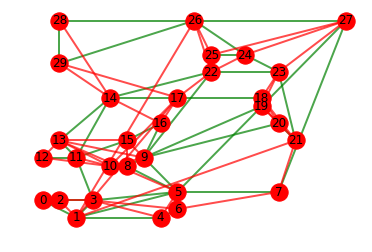
\includegraphics[width=.9\linewidth]{GridLayout.png}
	\caption{Overlaid power grid in green with road network in red}
	\label{fig:sub1}

\end{figure}

We also use the IEEE 57 test network, which has significantly more demand as it is loosely based on a representation of the American Midwest power grid in the 1960s. This test case from IEEE allows us to validate a larger network that has proportionally more demand and more complexity. 

\section{Geographically Clustered Damage}
Looking at our first case to validate the model, we manually apply geographically clustered damage to both road and power network. The damage in this case is concentrated where several damaged elements are next to each other in varying locations around the power grid. We show this in Figure 3.2 with damaged elements in red and operational elements in green. Of note here is that damaged substations have a damaged line close by.


\begin{figure}[htbp]
	\centering
	
	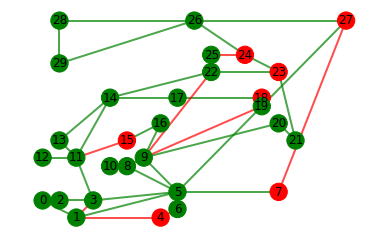
\includegraphics[width=.9\linewidth]{BaseCaseDamagePlot.png}
	\caption{IEEE 30 bus network with the base case damage applied and shown as red elements}
	\label{fig:sub1}
\end{figure}

For the base case on the 30 bus network, damage is applied to approximately one third of road segments, one quarter of power buses, and one third of power lines based on the damage modeling from the literature review. The following repair curves are generated from the model as stated earlier. This instance as well as all following instances are solved to a 1\% optimality gap. The reason for this is based on running instances, the final solution was found before this point.  

\begin{figure}[htbp]
	\centering
	
	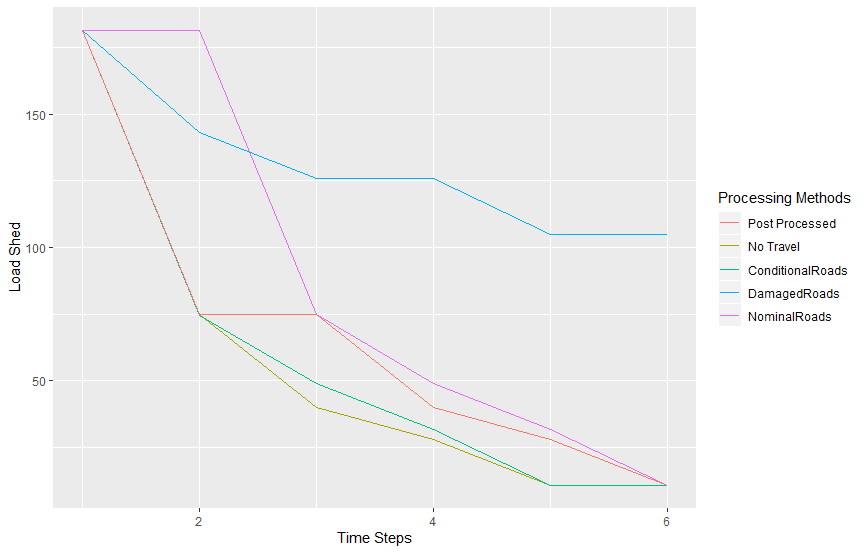
\includegraphics[width=.9\linewidth]{Rplot37.png}
	\caption{Load shed by shift in the 30 bus base instance}
	\label{fig:sub1}
\end{figure}
\begin{table}[htbp]
	\centering
	\caption{Total load shed over the repair horizon for the base instance}
	\resizebox{\columnwidth}{!}{\begin{tabular}{|c|c|c|c|c|}
	\hline	
	 Road First & Power First & Uncoordinated Repairs  &Post Processed & Lower Bound \\\hline
		291.7 & 479.4 & 291.7& 367.8 & 247.1 \\	
		\hline
	\end{tabular}}
	
	\label{time}
\end{table}
We conclude from Figure 3.3 as well as Table 3.1's summary of total unsatisfied demand across the repair horizon that changes in processing and interaction between models has meaningful impact on outcomes. It is worth noting that between points at the start and end of each shift, the shape of the repair curve is unknown. We present it as linear for the sake of simple visualization. For this case, we find that solving the roads and then conditioning the power repairs on that road schedule yields the outcome closest to the lower bound. This method being better is predicated on the assumption that the road repair crews would need one full shift to get ahead of what roads are needed in the framework where the power utility is the priority decision maker. If that delay can be reduced, letting the power utility dictate the road repair schedule becomes the best schedule inside the context of minimizing unsatisfied power demand over the repair horizon.


\section{Varied Damage location}
Looking at our next case to validate the models, we apply randomly distributed damage to both road network and power grid of similar intensity to the base case.
\begin{figure}[htbp]
	\centering
	
	\centering
	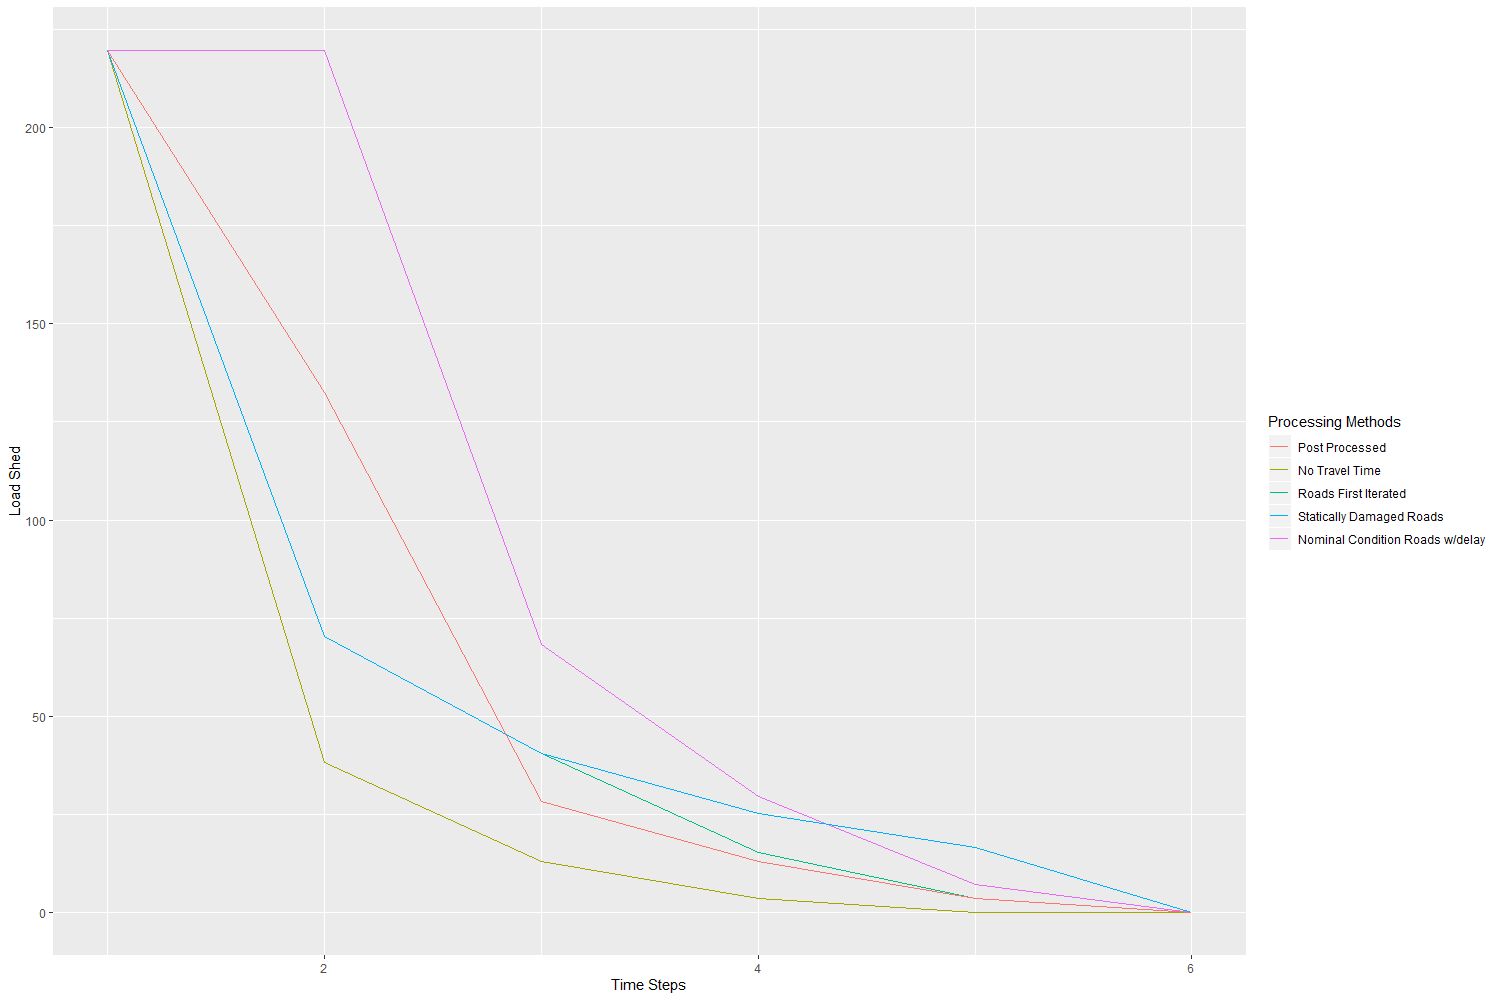
\includegraphics[width=.9\linewidth]{Rplot30Rand.png}
	\caption{Load shed by shift in the 30 bus randomized damage instance}
	\label{fig:sub1}
\end{figure}
\begin{table}[htbp]
	\centering
	\caption{Total load shed over the repair horizon for the random damage instance}
\resizebox{\columnwidth}{!}{\begin{tabular}{|c|c|c|c|c|}
		\hline	
		Road First & Power First & Uncoordinated Repairs  &Post Processed & Lower Bound \\\hline
		349.2 & 544.1 & 372.2 & 406.8 & 274.4\\	
		\hline
	\end{tabular}}
	
	\label{time}
\end{table}
We can draw comparable conclusions to the the geographically distributed base case, but for this instance as depicted in Figure 3.4 and Table 3.2. These repair curves having a rapid drop in load shed is due to the first several node and edge repairs being obvious choices. Given the rapid drop to baseline, the total lost load over the repair horizon is $544.8$ MW-shifts under the power first with delay framework as compared to the $349.2$ MW-shifts when solving the roads first or the $274.4$ MW-shifts of unsatisfied power demand in the lower bound solution. This is predicated on the delay to allow for road repairs to happen before they are needed for power grid repairs to occur with ideal transit times. Were this not to be the case, we find that the power first framework is the closest solution to the lower bound.

To demonstrate that the changes to how the road grid is treated drive much of the changes in satisfied power flow, we display the schedule for the random damage case in Table 3.3 for each of the interaction frameworks. The schedules are broadly similar in terms of what elements are prioritized, but by capturing the interactions with the road network, we can see that small perturbations to the schedule can dramatically change amount of demand unsatisfied over the repair horizon.

Of note is that not every element is repaired due to redundancies in the power grid, but that is justifiable in the context of disaster response as the first priority is satisfying demand and restoring redundant systems is a lower priority.  

\begin{table}[htbp]
	\centering
\caption{Repair schedule by interaction method for the 30 bus network with random damage}
	\begin{tabular}{|p{1.45cm}|p{2.1cm}|p{2.25cm}|p{2.5cm}|p{1.75cm}|p{1.75cm}|}
				
			\hline
			Shift Number & Road First & Power First & Uncoordinated Repairs  &Post Processed & Lower Bound \\\hline
			1 & Node 4, Line 2, Line 3 &Node 4, Line 2, Line 3, Line 17, Line 24& Node 4 and Line 3 & Node 7, Line 17, Line 3 & Node 4, Node 7, Line 3, Line 17 \\\hline
			2 & Node 7, Line 8, Line 35 & Node 7, Node 23& Node 7, Line 2, Line 24, Line 30,  & Node 4, Line 35&  Node 23, Node 24, Line 35\\\hline
			3 & Node 23, Node 24, Line 30 & Node 18, Node 24 & Node 15, Node 18, Line 17&  Node 23, Node 24 & Node 18, Line 2, Line 8, Line 20, Line 24, Line 30 \\\hline
			4 & Node 18, Line 14, Line 17, Line 24 & Node 20, Line 30, Line 35, Line 8, Line 14& Node 23, Line 8, Line 14, Line 35 & Node 18, Line 30, Line 2, Line 8, Line 20 & Node 15, Line 14\\\hline
			5 & Node 15, Line 20 & & Node 24 & Node 15, Line 24, Line 14&\\\hline
			6 & & & && \\\hline
	\end{tabular}
	
	\label{time}
\end{table}
\section{Varied Road Connectivity}
We now perturb the road topology of the network and solve a variation of the base case on the new road topology. The base-case road network was constructed as a Watts-Strogatz graph with neighbor connectivity 3 and global connectivity .03 as discussed earlier. To show the model as written is valid for multiple road topologies as well to show the impact of changing the road network, we permute the road network while keeping the power grid static. The new road topology is a different Watts-Strogatz graph with neighbor connectivity 2 and global connectivity .015. Additionally distances between nodes are increased by 25\%. This simulates the effect of the power grid in a more geographically spread out area with fewer direct paths between nodes.

The solutions are as follows in Figure 3.5 and 3.6 for first the unperturbed road network and then the perturbed road network. The damage here is another instance of random damage with a loss to 50\% of roads, 50\% of power lines, and 25\% of buses and substation in order to show the effects of a more severe hurricane and best the impact of the perturbed road network. 

\begin{figure}[htbp]
	\centering
	\includegraphics[width=.9\linewidth]{Rplot30unperturbed.png}
	\caption{Load shed by shift and method in a 30 bus instance before road perturbation}
	\label{fig:sub2}
	
	
\end{figure}
\begin{figure}[htbp]
	\centering
	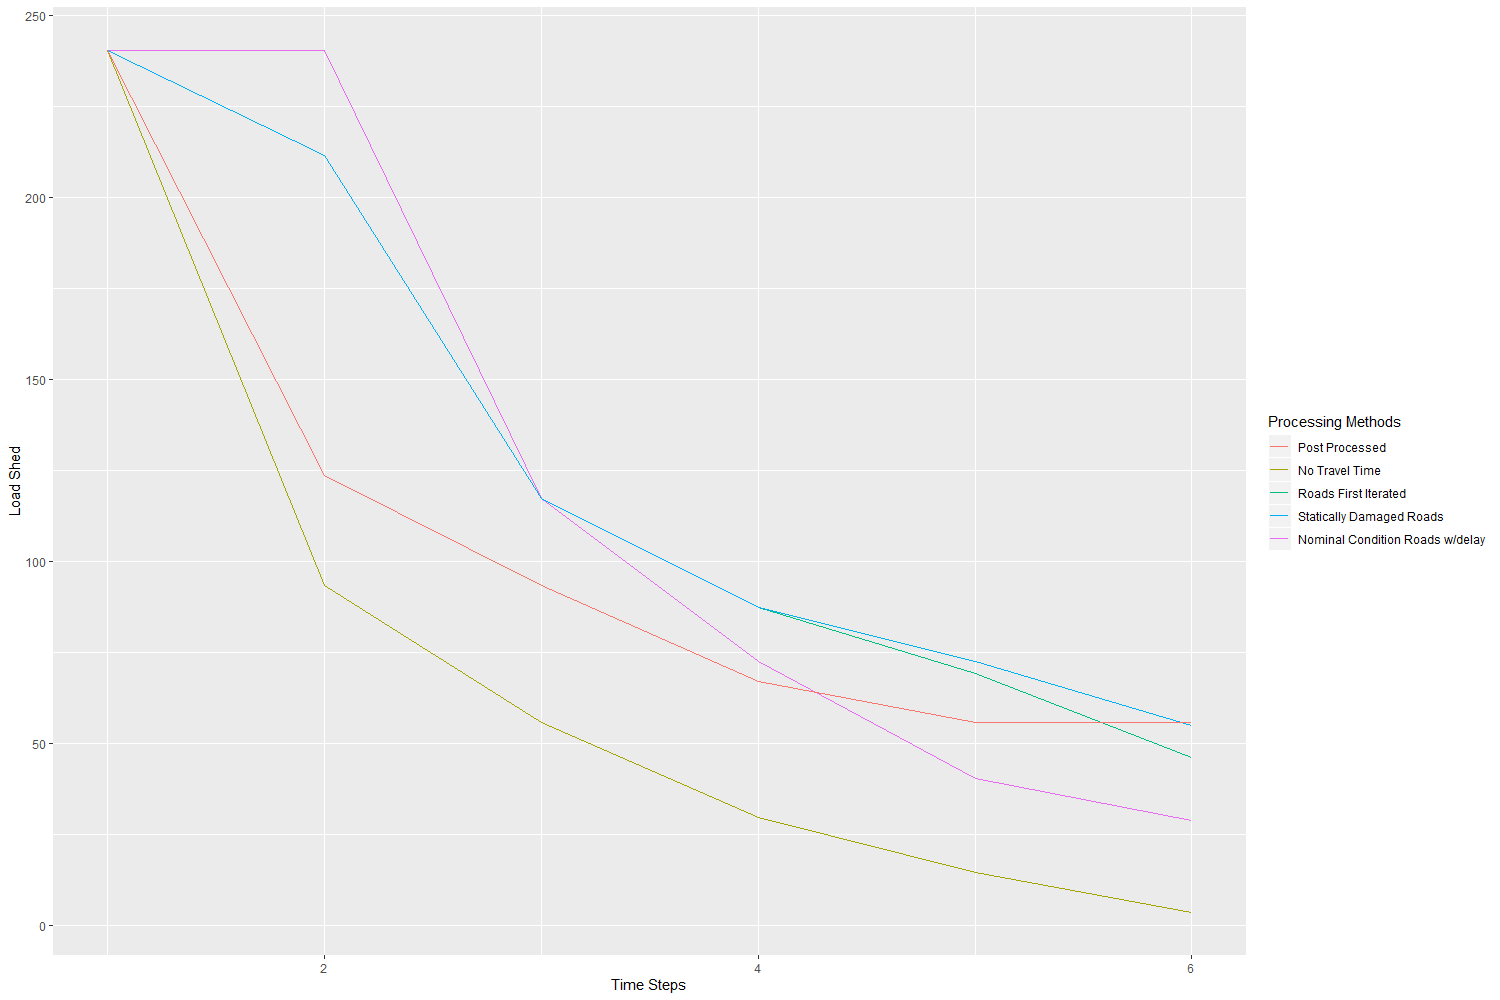
\includegraphics[width=.9\linewidth]{Rplot30Perturbed.png}
	\caption{Load shed by shift and method in a 30 bus instance for the geographically dispersed road network}
	\label{fig:sub2}
	
	
\end{figure}

We get largely intuitive changes here. Interaction frameworks that are on-face more sensitive to road changes (the uncoordinated repairs framework) have larger magnitudes of change in performance under perturbation of the road network. Figure 3.6 shows a markedly different curve set from Figure 3.5 where instead of a fairly steady decrease, we see a larger amount of damage carrying over into later parts of the repair horizon. Aditionally, there is far more deviation in framework solutions in the case where the roads are altered to be a more geographically distributed network. This is to be expected as more time within each shift is spent on the travel time causing fewer repairs to be done in each shift.

Of note here is that the heuristically solved version of the model without travel time and use of a post-processor performs much better (i.e closer to the lower bound) in the case with the road network perturbed to be more distant. This is  because the heuristic ignores road repair entirely in the name of not having to solve a mixed integer programming model. A version of the model where the road repair integer program is solved and used to generate time dependent road lengths for use in the post-processing heuristic would likely be significantly closer to the kind of solution the method would generate if deployed to real disaster response.

\section{Varied Damage Intensity}
We now perturb the base case for a higher damage instance in order to show model effectiveness for varying levels of damage. We show the higher damage in Figure 3.7
\begin{figure}[htbp]
	\centering
	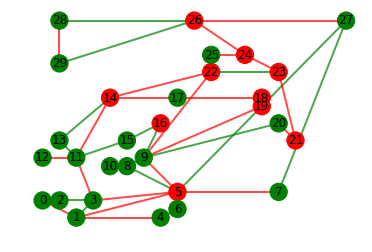
\includegraphics[width=.9\linewidth]{30BusSevereDamage.png}
	\caption{IEEE 30 bus network with the more severe damage applied and shown as red elements}
	\label{fig:sub2}
	
	
\end{figure}
\begin{figure}[htbp]
	\centering
	\includegraphics[width=.9\linewidth]{Rplot30scenario2.png}
	\caption{Load shed by shift in a 30 bus instance with increased damage}
	\label{fig:sub2}
	
	
\end{figure}
\begin{table}[htbp]
	\centering
	\caption{Total load shed over the repair horizon for the increased damage instance}
	\resizebox{\columnwidth}{!}{\begin{tabular}{|c|c|c|c|c|}
		\hline	
		Road First & Power First & Uncoordinated Repairs  &Post Processed & Lower Bound \\\hline
		447.9 & 548 & 454.2 & 477.7 & 327.9\\	
		\hline
	\end{tabular}}
	
	\label{time}
\end{table}

For larger amounts of damage on a network, the repair curve has a large initial drop followed by the similar amounts of tailing off seen in lower damage cases. This is because of most power grids having a few high priority node repair decisions for nodes that satisfy large amounts of the grid's demand. The remaining ~75MW of demand have less obvious decisions and depend more on the state of the road grid. This is seen clearly in Figure 3.8. While the post processed solution looks like it has a delay, but this is due to not fixing a particular node until the second shift and placing only line repairs in the first shift. We note here that uncoordinated repairs and solving the road repairs first generate the same repair curve. This is a consequence of the network having enough alternate routes that rerouting the repair crew does not alter the repair schedule. 
\section{Varied Grid Topology}
We now demonstrate the repair problem for a larger and more complex power grid in order to confirm model validity for larger scale problems. The road network is fit as it was for the base case where travel time from one side of the topology to the other is about 3 hours. We apply damage of comparable magnitude to the base case where damage is applied to approximately one third of road segments, one quarter of power buses, and one third of power lines
\begin{figure}[htbp]
	\centering
	\includegraphics[width=.9\linewidth]{Rplot57.png}
	\caption{Load shed by shift in the 57 bus instance}
	\label{fig:sub2}
	
	
\end{figure}

While the result for both solving the roads first and for solving with nominal condition roads with delay have similar behavior to previous cases' model interactions, the heuristic solution method of solving the lower bound and post-processing performs significantly worse. The reason for this is that a spatially larger power grid means that routing is a proportionally larger share of each shift, and ignoring that aspect until postprocessing results in solutions that get farther from the lower pound as the power grid grows spatially. In Figure 3.9, we see that both roads first and uncoordinated repairs framework have nearly the same load shed solution. This appears to be a flaw of how road damage is treated and suggests that a sparser road grid representation or higher proportion of road grid damage may be necessary to correctly capture the effects of road interactions for larger power grids.

\section{Model Runtimes}
Models are only useful if they can be implemented in a practical context. As disaster response planning is a somewhat time sensitive affair, a model that takes days or weeks to run is not useful as repairs need to start within the first few days. Based on using Gurobi 8.1.1 running on a i5-9600k CPU with 32gb of RAM running through the gurobipy interface for Python 3 for model building, model runtimes for road repairs range between 5 and 15 minutes on the 30 node case and 15-45 minutes on the 57 node case depending on the damage level. More damage leads to more possible decision options which means a longer runtime. Power repair model solution times range between 10-20 minutes for the IEEE 30 bus test network depending on interaction with the road network and 60-90 minutes for the IEEE 57 bus test network.


\section{Overall}
From the basket of demonstrated cases, we can see that interaction frameworks that allow more information sharing between road and power repairs are closer to the theoretical lower bound. As we make the assumption that power repairs that treat the road network as if it has been repaired to their needs requires a one shift delay in the start of repair operations, it is sub-par compared to solving the road network and then planning the power repairs based on that schedule. Were that assumption not to be valid, solving the power grid repairs under the presumption of nominal condition roads and then using those solutions to find a series of road repairs would be the best way of solving the repair problem if the only goal was to minimize total loss of satisfied demand in the power grid. Even with the delay, if the goal is to get the power grid back to nominal operation, solving the power first with the delay is better for higher damage cases. There are real reasons to give the road grid first-mover priority such as prioritizing flow in of humanitarian goods rather than restoration of power grid operations. Even under that interaction framework, power grid outcomes are better than they were under the schedule and post-process framework, suggesting that any coordination is still an improvement over methods that fail to capture the power/road interactions.


\section{Justifying the use of a Minimum Spanning Tree Approximation}

Now that we have presented several instances of the repair models, we can use these to go back and validate the use of our minimum spanning tree assumption when we first constructed the model.

In the above model we discuss the use of a minimum spanning tree to approximate the length of the route of a repair crew to reduce computational time. We demonstrate the validity of this by formulating the routing version of the problem, then running three instances to find first if we get the same (or at least a very similar) solution, and secondly to show the difference in runtime.

We begin by defining our sets and variables as above with the change that $Q_{ij}^t$ represents the inclusion of the shortest path from $i$ to $j$ in the tour at time $t$. We change $M^t$ from the length of the minimum spanning tree approximation of the route/tour length to the tour length itself. The routing model is then as follows:

\begin{equation}
\textnormal{Minimize}\sum_{i \in N} \sum_{t \in T} Y_{it}
\end{equation}
\textbf{subject to:}
\begin{eqnarray}
X_e^t = B_e (\theta_{o(e)}^t - \theta_{d(e)}^t), \hspace{5pt} \forall t \in T, \hspace{4pt} \forall e \in E\\
G_i^t - \sum_{e \in O(i)} X_e^t + \sum_{e \in D(i)} X_e^t = D_i-Y_i^t, \hspace{4pt} \forall t \in T, \hspace{4pt} \forall i \in N\\
0\leq G_k^t \leq P_{k} V_{k}^t, \hspace{4pt} \forall t \in T, \hspace{4pt} \forall k \in N\\
0\leq Y_i^t \leq D_i, \hspace{4pt} \forall t \in T, \hspace{4pt} \forall i \in N\\
-\overline{L_e}W_{e}^t \leq X_{e}^t \leq \overline{L_e}W_{e}^t, \hspace{4pt} \forall t \in T, \hspace{4pt} \forall e \in E\\
-\overline{L_e}V_{o(e)}^t \leq X_{e}^t \leq \overline{L_e}V_{o(e)}^t, \hspace{4pt} \forall t \in T, \hspace{4pt} \forall e \in E\\
-\overline{L_e}V_{d(e)}^t \leq X_{e}^t \leq \overline{L_e}V_{d(e)}^t, \hspace{4pt} \forall t \in T, \hspace{4pt} \forall e \in E\\
V_i^t \leq \sum_{t'=0}^{t-1} Z_i^{t'}+I_i, \hspace{4pt} \forall i \in N, \hspace{4pt} \forall t\in \{1,2,....t_{max}\}\\
W_{e}^t \leq \sum_{t'=0}^{t-1} U_{e}^{t'}+I_e, \hspace{4pt} \forall e \in E, \hspace{4pt} \forall t\in \{1,2,....t_{max}\}\\
M^t = \sum_{i \in N} \sum_{j \in N} {SP}_{ij}^t Q_{ij}^{t},  \hspace{4pt} \forall t \in T\\
\sum_{j \in N} Q_{ij}^t \geq Z_i^t, \hspace{4pt} \forall i \in N, \hspace{4pt} \forall t \in T\\
\sum_{j \in N} Q_{o(e)j}^t + \sum_{j \in N} Q_{d(e)j}^t \geq U_e^t, \hspace{4pt} \forall e \in E, \hspace{4pt} \forall t \in T\\
\sum_{j \in N} Q_{ij}^t - \sum_{j \in N} Q_{ji}^t = 0, \hspace{4pt} \forall i \in N, \hspace{4pt} \forall t \in T\\
\sum_{i,j \in S} Q_{ij}^t \leq |S|-1, \hspace{4pt} \forall S \subset N, \hspace{4pt} \forall t \in T\\
\sum_{e \in E} R_{e}U_e^t + \sum_{i \in N}R_{i}Z_i^t + M^t \leq F^t, \hspace{4pt} \forall t \in T\\
Q_{ij}^t,U_{e}^t,Z_{i}^t,W_{e}^t,V_{i}^t \in \{0,1\}. 
\end{eqnarray}

This model nearly the same as the model presented in Section 2.5, but the minimum spanning tree approximation to routing is replaced by a full routing problem in order to test the validity of the approximation we make. The changes are the replacement of constraints (2.31-2.33) in the original model with constraints (3.11-3.16). This more complex model generates the full route of the crew in terms of shortest paths between nodes rather than just determining what nodes they visit and providing a bound on what cost they pay to do so. 

We then solve a trio of instances check the validity of the minimum spanning tree assumption. Table 3.2 shows the optimum object function values and solution times of the corresponding models for the three instances. 
\begin{table}[htbp]
	\centering
	\caption{Runtime and objective values for minimum spanning tree and routing versions of the power repair problem}
	\resizebox{\columnwidth}{!}{\begin{tabular}{|c|c|c|c|c|}
			\cline{2-5}
			& \multicolumn{2}{c|}{MST} & \multicolumn{2}{c|}{Routing} \\
			\hline
			& MST Objective & MST Runtime & Routing Objective & Routing Runtime\\
			\hline
			Instance 1 (30 bus base instance)& $345.2$ & $25$ seconds   & $369.6$  & $639$ seconds  \\
			\hline
			Instance 2 (30 bus random damage instance) & $357.5$  & $15$ seconds & $406$ & $488$ seconds \\
			\hline
			Instance 3 (57 bus) & $2748$  & $4328$ seconds & no solution & $5400^*$ seconds\\
			
			\hline
	\end{tabular}}
	
	\label{time}
\end{table}

From this, we can see that the minimum spanning tree version of the model runs significantly faster and comes to a similar objective. The reason the 3rd instance has no solution for the routing based model is that these instances were run with a $90$ minute maximum runtime. At $90$ minutes, there was still a $22\%$ gap between the best incumbent solution and the lower bound solution in the branch-and-bound solver. While the second instance has a difference of 13.5\% between the objectives, the difference here is because of a single repair being moved to a later shift as a byproduct of the MST based model underestimating travel time. This leads us to believe this is an approximation that will be useful in planning disaster response. The step that would have to exist if the MST approximation is used is to solve the routing problem for the response crew between the selected elements. Determining the optimal route between less than 10 elements chosen for a shift by the MST based model is a simple and well solved problem.

	
	\chapter{Resilience}
\index{Resilience@\emph{Resilience}}%
\section{Introduction}
Given that we have constructed models for response to a scenario of a hurricane strike on power and road infrastructures, we can use these to look at how different methods of resilience interact with repair. We define resilience as the ability to withstand disruption and efficiently return to normal operation, but there are many definitions of resilience throughout literature on network operations \cite{MolyneauxEA2016}. In this chapter, we consider increasing the grid's resilience through hardening and fortification rather than an islanding based approach. We can then look to the repair procedures to evaluate the resilience of the power grid through looking at the rate of repair rather than just looking at the time to resume normal operation or magnitude of maximum initial drop in performance.

Most approaches to resilience construct a resilience curve such as the one in Figure 4.1  taken from \cite{Madni2020}. Resilience is shown as an initial drop and then time to both partial and full recovery.

\begin{figure}[htbp]
	\centering
	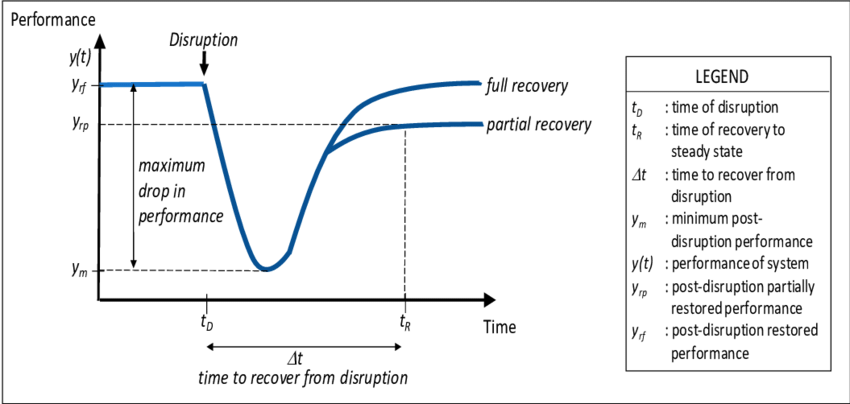
\includegraphics[width=.9\linewidth]{resiliencecurve.png}
	\caption{Standard depiction of a resilience curve}
\end{figure}

Large sections of the literature assume the recovery process for a system is fixed, so they study resilience in the context of minimizing either time to restoration of nominal system performance or minimizing the magnitude of the initial drop. We can frame this in terms of looking at the means versus the end. The goal is not to minimize some metric of resilience, but rather to reduce the impact of damage to the power grid. As we have been working with models for repair of damaged networks that generate repair schedules and associated curves showing power demand shed over time, we can look at all aspects of the resilience curve. This method gives us both the magnitude of the initial drop and the time to recovery in addition to the repair curve generated. Using this, we look into how the repair model defined above interacts with standard methods of improving resilience of a power grid.

\section{Hardening}

Hardening is one of the approaches to resilience achieved by fortifying a subset of nodes and edges in a network to make the network harder to damage. In the context of a power grid, this can include placing additional support guide wires on power poles, burying lines, or building flood walls and windbreakers around substations. Hardening is often looked at in the context of interdiction problems \cite{ChurchEA2007}.

 To overview the problem solved in interdiction: player 1 operates a network, player 2 attacks the network with the objective of maximizing demand shed under optimal power grid operation, and player 1 hardens the network before the attack under the assumption that it is coming and wants to preserve as much of the network's capacity as possible given a budget for hardening. This can be formulated as a trilayer maximization/minimization/maximization mixed integer programming \cite{Mahmoo2016}. Alternatively, it can be approached as a stochastic problem with uncertainties used to model attacks not being guaranteed to succeed \cite{Ramirez2009}.

A similar approach can be taken with disaster planning. Unlike in interdiction, the attack coming from a hurricane is a semi-random process of nature and not a targeted interdiction by an intelligent actor. Therefore the exact methods from directed attack based interdiction can not be implemented for models with more layers of decisions past attack and hardening. When solving this problem, we find a fixed quantity of damage based on the amount of hardening that can be undertaken with a budget constraint. By solving the ensuing interdiction problem, choosing the combination of elements that would be damaged forms the best set of elements to harden against damage. Solving this to optimality with best practices requires a delve into bi-level optimization that is outside the scope of this thesis. We therefore solve the problem heuristically through the following setup.

\begin{enumerate}
	
	\item Solve the baseline DC-OPF model for the given power grid
	\item Identify how many nodes (N) and edges (E) that are to be hardened based on the budget constraint
	\item Select at least the 2N highest demand nodes and the 2E highest utilization edges based on the DC-OPF model
	\item For each possible subset of N nodes and E edges, solve DC-OPF with those elements damaged (i.e down)
	\item Out of all the tested subsets, find the one that produces the maximum load shed in the DC-OPF solution. Use that subset of nodes and edges as the best choice for hardening when analyzing resilience.
\end{enumerate}

This is a heuristic solution rather than guaranteed optimality as written. In the case where all possible subsets are considered, this method generates a full solution to the multilayer (maximization of the minimum) optimization problem through enumeration. The result of this is a set of power grid elements that, if damaged, would maximally impede the operation of the power grid. The implication then is that by protecting this set of elements, the grid would be best protected against the worst case. This is the approach that Salmeron et al. \cite{Salmeron2004} took when studying terror attacks in the context of power grid resilience.
\section{Modeling}
We elect to use the IEEE 30 bus network outlined in earlier chapters to demonstrate the effectiveness of interdiction and priority heuristic based resilience procedure. Each scenario is solved three times using the interaction framework of solving the road grid first and then solving power grid repair based on that road repair schedule as laid out in Chapters 2 and 3. We solve for resilience in three ways:
\begin{itemize}
	\item Choosing hardened elements based on the interdiction method defined above
	\item Choosing hardened elements heuristically where the highest demand nodes and the edges that have the highest ratio of flow compared to their maximum flow limit. This is the kind of approximation that a power utility may use to choose elements to harden.
	\item Choosing no elements to be hardened
\end{itemize}.


Solution for the interdiction based hardening is done to optimality by selecting every subset of the desired size. The runtime for doing this is about 90 minutes because the model for load shed is a linear program and solves efficiently. The literature base on interdiction will have more sophisticated models and metaheuristics to solve or approximate interdiction on larger networks, but they are unnecessary for grids of this size since the optimal solution can be found with this simpler method.

We show the chosen hardened elements in Table 4.1 with the grid topology shown in Figure 4.2 for clarity as to what's hardened. Were all the elements from the interdiction based hardening method to be damaged, $233.4$ MW of demand would have to be shed. For the priority heuristic based method's chosen elements being damaged, the power grid would have to shed $187.6$ MW of demand.
\begin{figure}[htbp]
	\centering
	\includegraphics[width=.75\linewidth]{IEEE30layout.png}
	\caption{Layout of the power grid used for hardening and resilience}
\end{figure}

\begin{table}[htbp]
	\centering
	\caption{Hardened elements by resilience method }
	\resizebox{\columnwidth}{!}{\begin{tabular}{|c|c|c|}
			\hline	
			 & Interdiction Based & Priority Heuristic Based \\\hline
			Nodes & 1 and 7 & 4 and 7\\
			\hline
			Edges & (22,23), (5,9), (1,5), and (0,1)  & (22,23), (5,9), (23,24), and (14,17)\\
			\hline
	\end{tabular}}
	
	\label{time}
\end{table}

 We solve 20 repair problems corresponding to scenarios that are generated by uniform random generation are solved. Each scenario reflects 50\% line loss and 25\% bus loss in the power grid and a standardized road damage of 50\%. We solve the repair problem and find a schedule that will display the difference in not just recovery time, but amount of unsatisfied demand during the repair process for different treatments of resilience. In addition to this, we assess the objective with perfect information to construct a lower bound on the amount of demand unsatisfied in each scenario.

\subsection{Objective with Perfect Information}

 On top of these three methods of comparison in resilience, we also look at a case where we had perfect information about upcoming damage to generate a lower bound to compare to. If we knew which scenario will be realized, then the hardening of the most important elements for that scenario would be the optimal thing to do beforehand. Hardening here occurs with the same budget as the other methods. This method with perfect information is similar to wait-and-see lower bounds in optimization under uncertainty.
 
To assess the objective with perfect information, we construct a simple mixed integer program based on models presented earlier to identify that given we know exactly what damage is about to occur, what elements should be hardened. We formulate it as follows:

\begin{displaymath}
\begin{array}{ll}
N & \mbox{set of nodes, indexed by $i$} \\
E & \mbox{set of power lines, indexed by $e$}\\
O(i) & \mbox{set of lines with origin $i$} \\
D(i) & \mbox{set of lines with destination $i$} \\
o(e) & \mbox{origin node of line $e$} \\
d(e) & \mbox{destination node of line $e$} \\
\underline{L_e},\overline{L_e} & \mbox{power lower and upper bounds for line $e$}\\
D_i & \mbox{power demand in megawatts at node $i$ in the pre-disaster state}\\
P_k & \mbox{maximum power generation in megawatts for the generator at node $k$}\\
B_e &  \mbox{line susceptance in per unit siemens for power line $e$}\\
I_e, I_i & \mbox{a scenario's damage is represented here by $I_e$ and $I_i$ where 1 is working }\\
K_n & \mbox{The maximum number of nodes that can be hardened}\\
K_l & \mbox{The maximum number of edges that can be hardened}\\
X_{e} & \mbox{power flow in megawatts on line $e$}\\
G_{k} & \mbox{production from the generator at node $k$}\\
Y_{n} & \mbox{Load shed in megawatts from bus $n$}\\ 
V_i & \mbox{indicator for node $i$ being operational (1 is working) }\\
W_{e} & \mbox{indicator for line $e$ being operational (1 is working) }\\
U_{e} & \mbox{indicator for line $e$ being chosen to be hardened}\\
F_i & \mbox{indicator for node $i$ being chosen to be hardened}\\
\theta_i & \mbox{phase angle in radians for the power flow at node $i$}\\

\end{array}
\end{displaymath}
\begin{equation}
\textnormal{Minimize} \sum_{i \in N}  Y_i
\end{equation}
\textbf{subject to:}
\begin{eqnarray}
X_e = B_e (\theta_{o(e)} - \theta_{d(e)}),  \hspace{4pt} \forall e \in E\\
G_i - \sum_{e \in O(i)} X_e + \sum_{e \in D(i)} X_e = D_i-Y_i, \hspace{4pt} \forall t \in T, \hspace{4pt} \forall i \in N\\
G_k \leq P_{k} V_{k}, \hspace{4pt} \forall k \in N\\
0\leq Y_i \leq D_i, \hspace{4pt} \forall t \in T, \hspace{4pt} \forall i \in N\\
\underline{L_e}W_{e} \leq X_{e} \leq \overline{L_e}W_{e}, \hspace{4pt} \forall e \in E\\
\underline{L_e}V_{o(e)} \leq X_{e} \leq \overline{L_e}V_{o(e)},  \hspace{4pt} \forall e \in E\\
\underline{L_e}V_{d(e)} \leq X_{e} \leq \overline{L_e}V_{d(e)}, \hspace{4pt} \forall e \in E\\
V_i \leq F_i+I_i, \hspace{4pt} \forall i \in N\\
W_{e} \leq  U_{e}+I_e, \hspace{4pt} \forall e \in E\\
\sum_{i \in N} F_i \leq K_n\\
\sum_{e \in E} U_{e} \leq K_l\\
-\pi/2 \leq \theta_i \leq \pi/2, \hspace{4pt} \forall i \in N\\
S_{e}^t,F_{i}^t,W_{e}^t,V_{i}^t \in \{0,1\}. 
\end{eqnarray}

This is a variation on DC optimal power flow from Chapter 2 with load shedding. The objective is to minimize unsatisfied demand by choosing what elements to harden if we know the exact damage ahead of time. Constraints (4.9-4.12) handle the choice of hardening if the damage to the power grid is known ahead of time. While this is not a problem that will ever occur without weather modeling getting dramatically better, it is useful for generating a lower bound on damage such that a resilience strategy can be compared to both upper (do nothing) and lower (perfect information) bounds.

\section{Results}

We begin by showing the expected load shed across the full suite of 20 scenarios with equal weights on each scenario. We solve this by generating a scenario and computing the set of elements to harden with perfect information. Following this, the repair problem with the road first interaction framework is solved four times corresponding to each method of looking at resilience.  It is worth noting that averaging ``smooths out" the effect of individual scenarios, so several specific scenarios are displayed to make clear what the difference in a single scenario's actualization can be. The averages are shown in Figure 4.3 for hardening of two nodes and four edges.	
\begin{figure}[htbp]
	\centering
	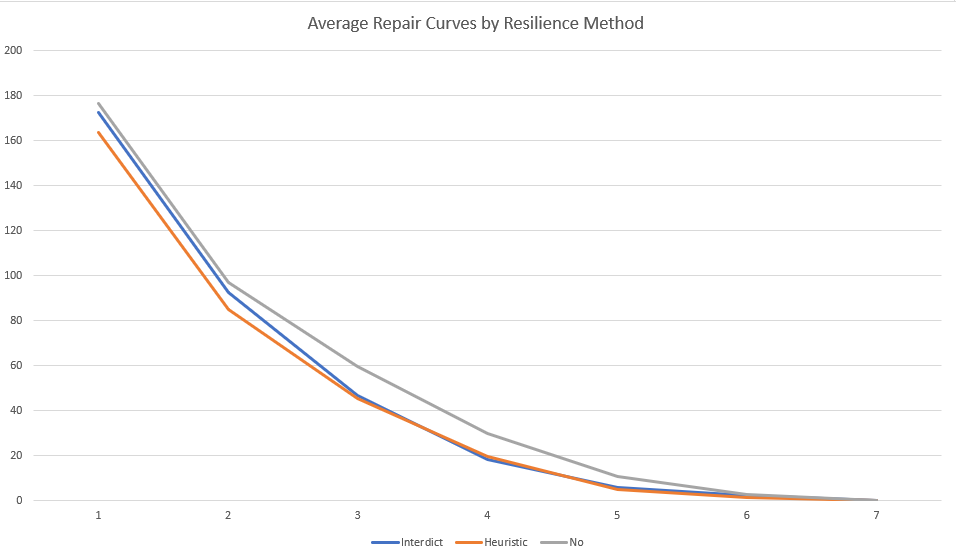
\includegraphics[width=.9\linewidth]{AverageSpaghetti.png}
	\caption{Average load demand shed over the set of 20 random scenarios on IEEE  30 bus}
\end{figure}

\begin{table}[htbp]
	\centering
		\caption{Expected unsatisfied demand by shift in each hardening method}
	\resizebox{\columnwidth}{!}{	\begin{tabular}{|c|c|c|c|c|}	
		\cline{1-5}
		Shift Number & Interdiction Based & Priority Heuristic Based & No Resilience & Perfect Information\\\hline
		1 & 168.3 & 171.5 & 187.9 & 107.4\\\hline
		2 & 74.7 & 92.1 & 100.9 & 39.9\\\hline
		3 & 41.1 & 43.3 & 53.1 & 15.3\\\hline
		4 & 14.8 & 18.3 & 28.3 & 4.54\\\hline
		5 & 4.3 & 4.1 & 9.5 & 0.24\\\hline
		6 & 1.3 & 1 & 2.0 & 0\\\hline
		7 & 0 & 0.12 & 0 & 0\\\hline
		total & 304.7 & 330.4 & 381.8 & 167.3\\\hline
	\end{tabular}}

	\label{time}
\end{table}


When using the interacted models to look at resilience though the repair curve, we find that over the average of the set of random scenarios modeled, interdiction based resilience has lower total expected load shed as well as a smaller expected initial drop. Figure 4.3 provides a visualization of this where the interdiction based method is visibly better than both the heuristic method and doing nothing. Both methods of making the power grid resilient are substantially better than doing nothing as would be intuitively expected, but the difference between use of the priority heuristic and solution to the full interdiction method is much smaller. This is still in line with expectations that more involved modeling should result in a better solution. Table 4.1 shows the direct magnitude where interdiction-based modeling results in the satisfaction of an additional 25 MW-shifts of demand. This small difference is due to interdiction models being best used for planned intelligent attacks and being and imperfect tool for planning hardening for random process.

We then break out the following two specific scenarios to showcase the effect that hardening an element matters most when it would be damaged by the disaster. Figure 4.4 shows the impact of protection of node 4 and several important lines by the priority heuristic based method that were not protected in the interdiction method. In this scenario, node 4 would have been damaged, but wasn't in the priority heuristic method because of hardening. This is not evidence that the heuristic is better than the interdiction method, but it does show the importance of hardening nodes that take damage. By contrast, Figure 4.5 shows a scenario where node 7 would have been damaged, but was not damaged due to hardening in all hardening cases. The differences in repair curves stem from the difference in hardened lines, showing that protection of nodes is not the only factor that matters. 

\begin{figure}[htbp]
	\centering
	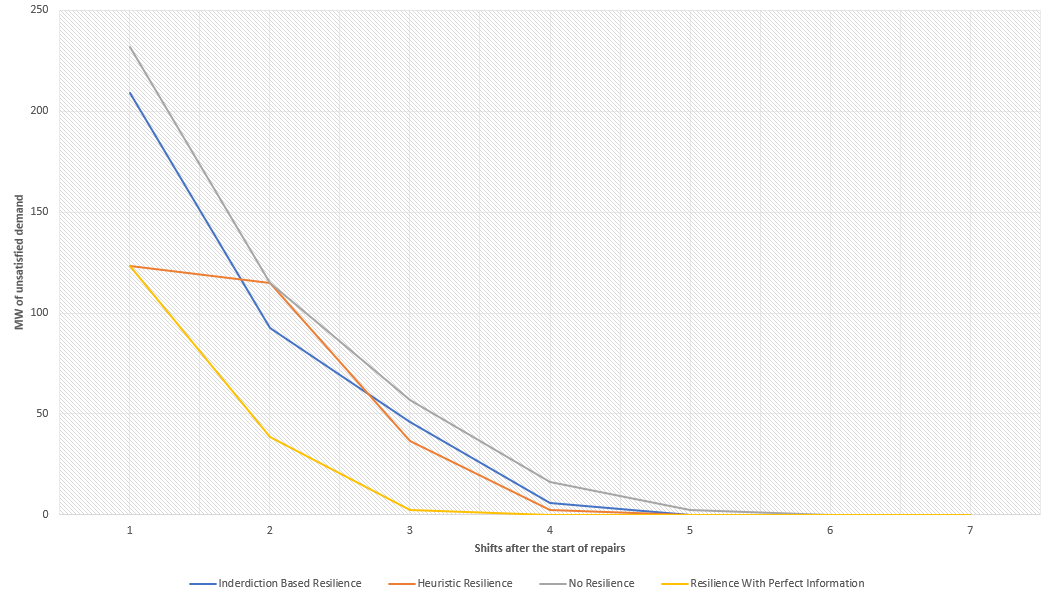
\includegraphics[width=.9\linewidth]{Heuristic24Scenario.png}
	\caption{A specific scenario from resilience modeling that shows the effect of protecting node 4 in the priority heuristic method}
\end{figure}
\begin{figure}[htbp]
	\centering
	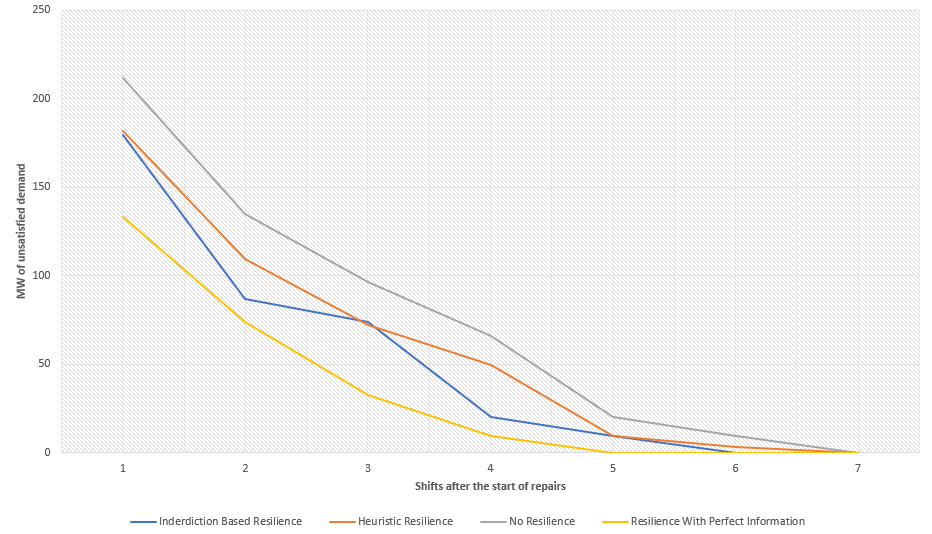
\includegraphics[width=.9\linewidth]{Inderdiction24Scenario.png}
	\caption{A specific scenario from resilience modeling that shows the effect of protecting damaged lines in the interdiction based method}
\end{figure}

Out of concern that the earlier results could be anomalous due to the budget constraint or grid topology based on choices of what elements to fortify, we repeat the process under a different budget constraint. We elect this time to fortify only one node and three edges to show the impact of a reduced budget. In the interdiction based method, we choose node 1 and edges (1,5), (22,23), and (0,1) for the interdiction based hardening. The priority heuristic hardens node 4 and edges (22,23), (22,24), and (5,9). We again create 20 random damage scenarios with the same parametersas before.
\begin{figure}[htbp]
	\centering
	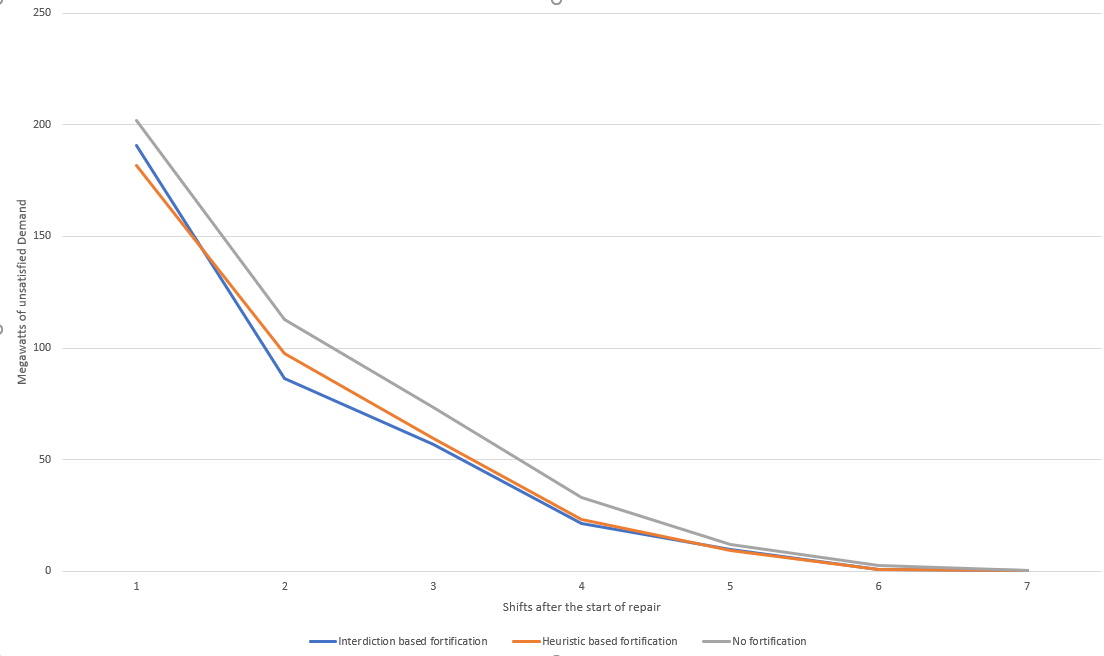
\includegraphics[width=.9\linewidth]{LowBudgetSpaghetti.png}
	\caption{Average repair curve for the tightened budget constraint}
\end{figure}
\begin{table}[htbp]
	\centering
		\caption{Expected unsatisfied demand by shift across resilience methods for a reduced hardening budget}
	\resizebox{\columnwidth}{!}{\begin{tabular}{|c|c|c|c|c|}
			\cline{1-5}
			Shift Number & Interdiction Based & Priority Heuristic Based & No Resilience & Perfect Information\\\hline
			1 & 192.2 & 184.8 & 201.4 & 127.6 \\\hline
			2 & 100.6 & 103.1 & 118.1 & 82.9 \\\hline
			3 & 64.7 & 61.8 & 76.0 & 43.0\\\hline
			4 & 25.6 & 25.4 & 35.7 & 19.5\\\hline
			5 & 12.1 & 10.6 & 13.3 & 5.12\\\hline
			6 & 1.85 & 1.21 & 2.75 & 0.83\\\hline
			7 & 0.22 & 0.22 & 0.33 & 0\\\hline
			total & 397.3 & 387.2 & 447.6 & 278.9\\\hline
	\end{tabular}}

	\label{time}
\end{table}

On the reduced budget, we see a similar conclusion to the higher budget example of resilience modeling when analyzing both Figure 4.6 and Table 4.3. In this case, the priority heuristic generates a slightly better solution in terms of both magnitude of initial drop and total lost load over the repair horizon. The reason for this is that interdiction based modeling can capture interactions between sets of elements. With only one node chosen, the impact of considering interactions rather than just heuristically choosing high priority elements is minimized. 

The conclusion from these two example studies into resilience is that the shape of the repair curves matter in terms of the end goal for resilient operations of power grids.  Changes in the curve shape leads to the difference in outcomes for the methods of choosing hardened elements on a power grid topology. Use of the repair curve captures both initial magnitude of damage as well as time to recovery when solving the optimal repair problem. As we see from comparing the interdiction based hardening to the priority heuristic solved hardening method, initial drop and time to resume nominal operations are not the only things that matter. Since interdiction based hardening is most frequently used in defense of a network against a directed attack and not a random event like a hurricane, it may not be the best tool for the job in planning resilience against a random event. We suspect this to be a place where probability based resilience methods based on hardening/fortifying the elements most likely to be damaged based on assessment of hurricane forecasts or some form of two step stochastic optimization to construct a resilience plan would be the best approach to take. 


	
	\chapter{Conclusions}
\index{Conclusions@\emph{Conclusions}}%

	\section{Conclusions}

As discussed in the literature review, interaction between actors in a repair context has not been thoroughly explored. We present a pair of models and analyze several perturbations of standard IEEE test grids to demonstrate the effectiveness of interacting the models in several different frameworks. This yields a series of results that are closer to a theoretical lower bound as compared to treating repairs as a pure scheduling problem on the power grid and applying routing as an after-the-fact post processing step as is done in previous modeling efforts that generate only a schedule and leave routing to the agency conducting repairs.

These repair models are then extended into resilience models to show that interdiction based modeling performs better than a heuristic method at minimizing the unsatisfied power demand over a basket of random damage instances. This suggests that further consideration of multiple network layers can lead to better insights when considering resilience planning of multiple network layers.


\section{Future Research Directions}
The natural extensions for future research are to take the models outlined and fit them to the topology of a real place that is struck by hurricanes such as Houston and then simulate a hurricane strike to generate the damage scenario. This would require an involved effort to correctly model both flooding/storm surge as well as wind damage, but is possible. Additionally along the same line of research, treating the repair problem outlined above as a recourse step in a two stage stochastic program based on a suite of hurricane scenarios would be an interesting direction of study. The first step could take the form of inventory location and quantity or problem about network hardening.

Another research direction that could be undertaken is to account for imperfect information about the state of the power grid or imperfect information about the status of the road network. Sharing of resources (e.g space on a truck moving supplies in) as a form of optimization under uncertainty which would also have implications for interesting interactions between decision makers in the repair effort. Along those lines, optimization of roads has implications for other types of network infrastructure such as water supplies and rail/mass transit networks.
	
	
	
	%%%%%%%%%%%%%%%%%%%%%%%%%%%%%%%%%%%%%%%%%%%%%%%%%%%%%%%%%%%%%%%%%%%%%%
	% Appendix/Appendices                                                %
	%%%%%%%%%%%%%%%%%%%%%%%%%%%%%%%%%%%%%%%%%%%%%%%%%%%%%%%%%%%%%%%%%%%%%%
	%
	% If you have only one appendix, use the command \appendix instead
	% of \appendices.
	%

	
	%%%%%%%%%%%%%%%%%%%%%%%%%%%%%%%%%%%%%%%%%%%%%%%%%%%%%%%%%%%%%%%%%%%%%%
	% Generate the bibliography.					     %
	%%%%%%%%%%%%%%%%%%%%%%%%%%%%%%%%%%%%%%%%%%%%%%%%%%%%%%%%%%%%%%%%%%%%%%
	%								     %
	% NOTE: For master's theses and reports, NOTHING is permitted to     %
	%	come between the bibliography and the vita. The command      %
	%	to generate the index (if used) MUST be moved to before      %
	%	this section.						     %
	%								     %
	\nocite{*}      % This command causes all items in the 		     %
	% bibliographic database to be added to 	     %
	% the bibliography, even if they are not 	     %
	% explicitly cited in the text. 		     %
	%						     %
	\bibliographystyle{plain}  % Here the bibliography 		     %
	\bibliography{Sources}        % is inserted.			     %
	\index{Bibliography@\emph{Bibliography}}%			     %
	%%%%%%%%%%%%%%%%%%%%%%%%%%%%%%%%%%%%%%%%%%%%%%%%%%%%%%%%%%%%%%%%%%%%%%
	
	
	%%%%%%%%%%%%%%%%%%%%%%%%%%%%%%%%%%%%%%%%%%%%%%%%%%%%%%%%%%%%%%%%%%%%%%
	% Generate the index.						     %
	%%%%%%%%%%%%%%%%%%%%%%%%%%%%%%%%%%%%%%%%%%%%%%%%%%%%%%%%%%%%%%%%%%%%%%
	%								     %
	% NOTE: For master's theses and reports, NOTHING is permitted to     %
	%	come between the bibliography and the vita. This section     %
	%	to generate the index (if used) MUST be moved to before      %
	%	the bibliography section.				     %
	%								     %
	%\printindex%    % Include the index here. Comment out this line      %
	%		% with a percent sign if you do not want an index.   %
	%%%%%%%%%%%%%%%%%%%%%%%%%%%%%%%%%%%%%%%%%%%%%%%%%%%%%%%%%%%%%%%%%%%%%%
	
	
	%%%%%%%%%%%%%%%%%%%%%%%%%%%%%%%%%%%%%%%%%%%%%%%%%%%%%%%%%%%%%%%%%%%%%%
	% Vita page.							     %
	%%%%%%%%%%%%%%%%%%%%%%%%%%%%%%%%%%%%%%%%%%%%%%%%%%%%%%%%%%%%%%%%%%%%%%
	
	\begin{vita}
		Brian French
		was born in Detroit Michigan in 1995, the son of Dr. R. Mark French and Amy French.  He received a dual Bachelor of Science degree in both economics and mathematical statistics from Purdue University in 2018. he applied to the University of Texas at Austin for enrollment in their operations research and industrial engineering program. He was accepted and started graduate studies in August, 2018.
		
	\end{vita}
	
\end{document}
